\documentclass[12pt, a4paper]{article}

% Pacchetti fondamentali
\usepackage[utf8]{inputenc}
\usepackage[italian]{babel}
\usepackage{geometry}
\geometry{a4paper, top=3cm, bottom=3cm, left=2.5cm, right=2.5cm}
\usepackage{tabularx}
\usepackage{booktabs}
\usepackage{hyperref}
\usepackage{eurosym}
\usepackage{graphicx}
\usepackage{titlesec}
\usepackage[figure,table]{totalcount}
\usepackage{fancyhdr}
\usepackage{adjustbox}
\usepackage{extramarks}
\usepackage{makecell}
\usepackage{graphicx}
\usepackage{float}
\usepackage{xltabular}
\usepackage[skip=10pt plus 2pt, indent=5pt]{parskip}
\newcommand{\urlglossario}{https://skynetunigroup.github.io/Code_Guardian/Documentazione/PB/glossario_v2.0.0.pdf}
\newcommand{\glo}[2]{\href{\urlglossario\#nameddest=#2}{#1\textsubscript{G}}}

\pagestyle{fancy}
\fancyhf{}
\setlength{\headheight}{35pt}

% Setup dei link interattivi (indice)
\hypersetup{
    colorlinks=true,
    linkcolor=black,
    filecolor=magenta,      
    urlcolor=blue,
}

\newcommand{\doctitle}{Specifiche Tecniche} % Sostituisci con il titolo reale

% --- INTESTAZIONE (HEADER) ---
\lhead{\nouppercase{\firstleftmark}}
\rhead{\adjustbox{valign=m}{
\includegraphics[height=1cm]{logo_skynet_dark.png}}}

% --- PIÈ DI PAGINA (FOOTER) ---
\lfoot{\doctitle} 
\rfoot{\thepage} 

% Linee di separazione
\renewcommand{\headrulewidth}{0.4pt} % Linea sotto l'intestazione
\renewcommand{\footrulewidth}{0.4pt} % Linea sopra il piè di pagina

\begin{document}

% ==========================================
% FRONTESPIZIO
% ==========================================
\begin{titlepage}
    \centering
    
\includegraphics[width=0.5\linewidth]{logo_skynet_dark.png}
    
    {\Large Gruppo SkyNet}\\
    {\normalsize \href{mailto:skynetunigroup@gmail.com}{skynetunigroup@gmail.com}}
    \vspace*{1.5cm}
    
    {\Huge \textbf{\doctitle}} \\
    
    \vspace{3cm}
    
    % Tabella Informazioni Documento, sostituire con il contenuto reale
    \begin{table}[h]
        \centering
        \renewcommand{\arraystretch}{1.5}
        \begin{tabularx}{\textwidth}{|l|X|}
            \hline
            \textbf{Versione} & \textit{1.0.0} \\ \hline
            \textbf{Uso} & \textit{Esterno} \\ \hline
            \textbf{Destinatari} & \textit{Prof. Tullio Vardanega, Prof. Riccardo Cardin} \\ \hline
            \textbf{Redattori} & \textit{Sara Ristovic, Dario Pirrone, Edoardo Granziero} \\ \hline
            \textbf{Verifica} & \textit{Marco Barbiero, Dario Pirrone, Sara Ristovic, Edoardo Granziero} \\ \hline
            \textbf{Approvazione} & \textit{Marco Barbiero} \\ \hline

        \end{tabularx}
    \end{table}
    
    \vfill
\end{titlepage}
\stepcounter{page}

\newpage

% ==========================================
% REGISTRO DELLE VERSIONI
% ==========================================
\section*{Versioni del documento}
\markboth{Versioni del documento}{}
{\renewcommand{\arraystretch}{1.3}
\begin{xltabular}{\textwidth}{|c|c|X|p{2.2cm}|p{2.2cm}|}
    \hline
    \textbf{Ver.} & \textbf{Data} & \textbf{Descrizione} & \textbf{Autore} & \textbf{Verificatore} \\ \hline
    \endfirsthead
    
    \hline
    \textbf{Ver.} & \textbf{Data} & \textbf{Descrizione} & \textbf{Autore} & \textbf{Verificatore} \\ \hline
    \endhead
    
    1.0.0 & 2026/09/16 & Approvazione del documento per revisione PB & \makecell[l]{Marco \\Barbiero}& -- \\ \hline
    0.11.0 & 2026/09/15 & Lettura dell'intero documento e riscrittura di alcune parti per renderle più chiare e fluide  & \makecell[l]{Edoardo \\Granziero} & \makecell[l]{Sara \\Ristovic} \\ \hline
    0.10.0 & 2026/09/15 & Correzioni delle sezioni 1, 2 e 3 in seguito alla verifica & \makecell[l]{Sara \\Ristovic} & \makecell[l]{Edoardo \\Granziero} \\ \hline
    0.9.0 & 2026/09/15 & Correzione dei diagrammi e del testo nella sezione "Flusso dei dati" in seguito alla verifica & \makecell[l]{Dario \\Pirrone} & \makecell[l]{Sara \\Ristovic} \\ \hline
    0.8.0 & 2026/09/14 & Scrittura della sezione "Copertura dei requisiti" & \makecell[l]{Sara \\Ristovic} & \makecell[l]{Dario \\Pirrone} \\ \hline
    0.7.0 & 2026/09/13 & Scrittura della sezione "Flusso dei dati" & \makecell[l]{Sara \\Ristovic} & \makecell[l]{Dario \\Pirrone} \\ \hline
    0.6.0 & 2026/09/13 & Scrittura della sezione "Design Pattern Implementati" & \makecell[l]{Sara \\Ristovic} & \makecell[l]{Dario \\Pirrone} \\ \hline
    0.5.0 & 2026/09/11 & Scrittura della sottosezione "Architettura del Servizio Agenti" & \makecell[l]{Sara \\Ristovic} & \makecell[l]{Marco \\Barbiero} \\ \hline
    0.4.0 & 2026/09/06 & Scrittura delle sottosezioni Architettura di Deployment, del Frontend e del Backend; Scrittura della sottosezione "Modello dei Dati Persistiti" & \makecell[l]{Sara \\Ristovic} & \makecell[l]{Dario \\Pirrone} \\ \hline
    0.3.0 & 2026/09/03 & Scrittura della sottosezione "Vista d'insieme" & \makecell[l]{Sara \\Ristovic} & \makecell[l]{Dario \\Pirrone} \\ \hline
    0.2.0 & 2026/09/02 & Scrittura della sezione "Tecnologie" & \makecell[l]{Sara \\Ristovic} & \makecell[l]{Marco \\Barbiero} \\ \hline
    0.1.0 & 2026/09/01 & Strutturazione del documento e scrittura della sezione "Introduzione" & \makecell[l]{Sara \\Ristovic} & \makecell[l]{Marco \\Barbiero} \\ \hline
\end{xltabular}
}

\newpage
% ==========================================
% INDICI
% ==========================================
\tableofcontents
\iftotaltables  % Se sono presenti tabelle o figure appare l'indice
    \vspace{1cm}
    \listoftables
\fi

\iftotalfigures
    \vspace{1cm}
    \listoffigures
\fi
\newpage

% ==========================================
% CONTENUTO DEL DOCUMENTO
% ==========================================

\section{Introduzione}

\subsection{Scopo del documento}

Questo documento espone l'architettura logica dell'MVP \textbf{Code Guardian}: le componenti principali, le loro responsabilità e le connessioni tra di esse. Serve inoltre come riferimento per lo sviluppo successivo e per la manutenzione del prodotto. Al suo interno vengono dettagliate le tecnologie selezionate, descritta l'architettura di deployment, illustrati i design pattern adottati e analizzati altri aspetti progettuali di rilievo. L'ultima sezione riporta la copertura dell'implementazione dei requisiti stabiliti nella prima fase del progetto.
 
Lo abbiamo redatto a conclusione della progettazione architetturale, sintetizzando le parti salienti dei documenti di dettaglio su backend, frontend, infrastruttura AWS e servizio agenti. L'architettura definitiva resta coerente con quanto validato nel \textit{PoC}: le soluzioni tecniche e le componenti buone del prototipo sono state riprese.

\subsection{Scopo del prodotto}

\textbf{Code Guardian} è un'applicazione web che automatizza i processi di security audit, manutenzione e documentazione all'interno dei repository software. L'obiettivo è togliere ai team di sviluppo il lavoro manuale più ripetitivo, alzando allo stesso tempo il livello di sicurezza del codice e tenendo aggiornata la documentazione tecnica.

Al centro del prodotto c'è un orchestratore deterministico, che coordina l'attività di tre agenti intelligenti basati su LLM esterni:
\begin{itemize}
    \item \textbf{Agente Docs}: genera una proposta di aggiornamento del README di progetto in base alle effettive modifiche del codice sorgente, propone commenti inline standardizzati (Docstring per Python, JSDoc per TypeScript/JavaScript) e compila guide API allineate allo stato del software. Produce una proposta di modifica (diff), che il backend trasforma in una Pull Request quando applicabile: l'agente non scrive mai direttamente sui file del repository.
    \item \textbf{Agente Security}: esegue un'analisi semantica del codice per individuare le falle di sicurezza più critiche appartenenti alla classificazione OWASP Top 10. Applica inoltre il principio del Policy-as-code, verificando l'aderenza delle pratiche di scrittura del codice alle regole interne definite dal team nel file POLICY.md.
    \item \textbf{Agente Changelog}: si integra direttamente con \textit{GitHub Issues} per estrarre le attività completate durante uno \textit{sprint}. Traduce poi il gergo tecnico delle task in report chiari e leggibili, producendo sia un changelog di tipo ingegneristico per gli sviluppatori, sia un changelog orientato al business per i clienti e il management.
\end{itemize}

Il prodotto risponde alle esigenze di diversi tipi di utente:
\begin{itemize}
    \item \textbf{Sviluppatori}: beneficiano dell'allineamento automatico della documentazione.
    \item \textbf{Security Auditor}: ottengono una piattaforma per monitorare facilmente l'aderenza alle linee guida di sviluppo sicuro del team e agli standard di sicurezza.
    \item \textbf{Project Manager e Stakeholder di business}: possono seguire con trasparenza l'andamento reale dello sviluppo e i progressi di ogni \textit{sprint} senza dover possedere competenze tecniche avanzate.
\end{itemize}

\subsection{Riferimenti}
\subsubsection{Riferimenti normativi}
\begin{itemize}
\item
  \href{https://www.math.unipd.it/~tullio/IS-1/2025/Progetto/C2p.pdf}{Capitolato d'appalto C2 - \textbf{Code Guardian}} (\textit{Data ultimo accesso: 16/09/2026})
\item
  \href{https://www.math.unipd.it/~tullio/IS-1/2025/Dispense/PD1.pdf}{Regolamento del Progetto Didattico} (\textit{Data ultimo accesso: 16/09/2026})
  \item \href{https://skynetunigroup.github.io/Code_Guardian/Documentazione/PB/norme_di_progetto_v2.0.0.pdf}{\textbf{Norme di Progetto} v2.0.0}


\end{itemize}


\subsubsection{Riferimenti informativi}
\begin{itemize}
\item \href{https://skynetunigroup.github.io/Code_Guardian/Documentazione/PB/analisi_dei_requisiti_v2.0.0.pdf}{\textbf{Analisi dei Requisiti} v2.0.0}
\item \href{https://skynetunigroup.github.io/Code_Guardian/Documentazione/PB/glossario_v2.0.0.pdf}{Glossario v2.0.0}
\end{itemize}


\newpage
\section{Tecnologie}

Questa sezione elenca le tecnologie adottate per la release MVP, organizzate per ruolo. Per Backend e Frontend le versioni riportate sono quelle risolte in \texttt{pnpm-lock.yaml} alla data di redazione. Per gli Agenti non esiste invece un lockfile: \texttt{pyproject.toml} dichiara vincoli minimi (e in un caso un tetto massimo), non versioni risolte. Le versioni riportate per gli Agenti sono quindi i vincoli dichiarati, non un numero risolto.

\subsection{Linguaggi e Framework}

\renewcommand{\arraystretch}{1.3}
\begin{xltabular}{\textwidth}{|l|l|l|X|}
    \caption{Linguaggi e framework principali, per servizio}\label{tab:linguaggi-framework} \\
    \hline
    \textbf{Tecnologia} & \textbf{Versione} & \textbf{Servizio} & \textbf{Descrizione} \\ \hline
    \endfirsthead
    \multicolumn{4}{l}{\small\textit{(segue dalla pagina precedente)}} \\
    \hline
    \textbf{Tecnologia} & \textbf{Versione} & \textbf{Servizio} & \textbf{Descrizione} \\ \hline
    \endhead
    \hline
    \multicolumn{4}{r}{\small\textit{(continua nella pagina successiva)}} \\
    \endfoot
    \hline
    \endlastfoot
    TypeScript & 6.0.3 & \makecell[l]{Backend \\ Frontend} & Linguaggio principale. \\ \hline
    Node.js & 26 & Backend & Runtime JavaScript su cui gira il servizio NestJS in container. \\ \hline
    Node.js & 26 & Frontend & Runtime usato in fase di build dell'immagine Docker del Frontend. \\ \hline
    NestJS & 11.2.3 & Backend & Framework Backend, basato su Node.js/TypeScript. \\ \hline
    React & 19.2.8 & Frontend & Libreria per la costruzione dell'interfaccia utente. \\ \hline
    Python & $\geq$3.12 & Agenti & Linguaggio del servizio Agenti. \\ \hline
    FastAPI & $\geq$0.111.0 & Agenti & Framework web su cui è esposta l'API interna del servizio Agenti. \\ \hline
    Uvicorn & $\geq$0.30.0 & Agenti & Server \textit{\glo{ASGI}{asgi}} su cui gira FastAPI. \\ \hline
    LangGraph & $\geq$0.2.20 & Agenti & Framework di orchestrazione del grafo agente. \\ \hline
\end{xltabular}

\subsection{Librerie Frontend}

Librerie applicative usate dal Frontend oltre al framework React.

\renewcommand{\arraystretch}{1.3}
\begin{xltabular}{\textwidth}{|p{5.2cm}|l|X|}
    \caption{Librerie Frontend}\label{tab:librerie-frontend} \\
    \hline
    \textbf{Libreria} & \textbf{Versione} & \textbf{Descrizione} \\ \hline
    \endfirsthead
    \multicolumn{3}{l}{\small\textit{(segue dalla pagina precedente)}} \\
    \hline
    \textbf{Libreria} & \textbf{Versione} & \textbf{Descrizione} \\ \hline
    \endhead
    \hline
    \multicolumn{3}{r}{\small\textit{(continua nella pagina successiva)}} \\
    \endfoot
    \hline
    \endlastfoot
    Vite & 8.2.2 & Bundler e dev-server. \\ \hline
    @vitejs/plugin-react & 6.1.1 & Plugin ufficiale Vite per il supporto a React. \\ \hline
    \texttt{@tanstack/react-router} & 1.170.32 & Router con tipizzazione nativa di rotte e parametri. \\ \hline
    Zustand & 5.0.15 & Gestione dello stato globale applicativo (store). \\ \hline
    Tailwind CSS & 3.4.19 & Framework CSS utility-first, base del design system. \\ \hline
    \texttt{@tailwindcss/typography} & 0.5.20 & Plugin Tailwind per la tipografia dei contenuti Markdown renderizzati. \\ \hline
    \makecell[l]{\texttt{clsx} \\ \texttt{class-variance-authority} \\ \texttt{tailwind-merge} \\ \texttt{lucide-react}} & \makecell[l]{2.1.1 \\ 0.7.1 \\ 3.6.0 \\ 1.40.0} & Libreria di componenti accessibili: i componenti \texttt{shadcn/ui} vengono copiati direttamente nel codice sorgente del Frontend, non installati come pacchetto npm (\texttt{shadcn/ui} non compare quindi in \texttt{package.json}). Le quattro voci a sinistra sono invece le dipendenze reali che quei componenti importano, effettivamente installate. \\ \hline
    \texttt{react-markdown} / \texttt{remark-gfm} & 10.1.0 / 4.0.1 & Rendering dei blocchi di testo del report come Markdown, con supporto GitHub Flavored Markdown. \\ \hline
    Socket.IO Client & 4.8.3 & Client per il canale realtime verso il Backend. \\ \hline
    Axios & 1.20.0 & Client HTTP per le chiamate REST al Backend. \\ \hline
\end{xltabular}

\subsection{Librerie Backend}

Librerie applicative usate dal Backend oltre al framework NestJS.

\renewcommand{\arraystretch}{1.3}
\begin{xltabular}{\textwidth}{|p{5.2cm}|l|X|}
    \caption{Librerie Backend}\label{tab:librerie-backend} \\
    \hline
    \textbf{Libreria} & \textbf{Versione} & \textbf{Descrizione} \\ \hline
    \endfirsthead
    \multicolumn{3}{l}{\small\textit{(segue dalla pagina precedente)}} \\
    \hline
    \textbf{Libreria} & \textbf{Versione} & \textbf{Descrizione} \\ \hline
    \endhead
    \hline
    \multicolumn{3}{r}{\small\textit{(continua nella pagina successiva)}} \\
    \endfoot
    \hline
    \endlastfoot
    \texttt{mongoose} / \texttt{@nestjs/mongoose} & 9.9.4 / 11.0.4 & \textit{\glo{ODM}{odm}} per l'accesso a MongoDB, con il relativo modulo di integrazione NestJS. \\ \hline
    \texttt{@nestjs/jwt} & 11.0.2 & Emissione e verifica dei token \textit{\glo{JWT}{jwt}} di sessione. \\ \hline
    Passport / \texttt{passport-jwt} & 0.7.0 / 4.0.1 & Strategia di autenticazione basata su JWT. \\ \hline
    argon2 & 0.45.1 & Hashing delle password (Argon2id). \\ \hline
    class-validator / class-transformer & 0.15.1 / 0.5.1 & Validazione e trasformazione dei \textit{\glo{DTO}{dto}} in ingresso. \\ \hline
    Joi & 18.2.5 & Validazione delle variabili di configurazione/ambiente. \\ \hline
    \texttt{@nestjs/swagger} & 11.4.7 & Generazione della documentazione OpenAPI degli endpoint pubblici. \\ \hline
    \texttt{socket.io} / \texttt{@nestjs/platform-socket.io} & 4.8.3 / 11.2.3 & Canale realtime verso il Frontend, con il relativo adapter NestJS. \\ \hline
    \texttt{@octokit/rest} & 22.0.1 & Client per le chiamate all'API REST di GitHub. \\ \hline
    diff & 9.0.0 & Applicazione delle patch/diff proposte dagli agenti sui file. \\ \hline
    franc-min & 6.2.0 & Rilevamento della lingua del README, usato dall'Agente Docs. \\ \hline
    pdfkit & 0.20.2 & Composizione del PDF esportato di un Report. \\ \hline
    \texttt{@aws-sdk/client-s3} & 3.1127.0 & Caricamento degli artefatti (PDF esportati) su Amazon S3. \\ \hline
\end{xltabular}

\subsection{Persistenza e Caching}

Tecnologie di persistenza e caching condivise da Backend e Agenti.

\renewcommand{\arraystretch}{1.3}
\begin{xltabular}{\textwidth}{|p{5.2cm}|l|X|}
    \caption{Persistenza e caching}\label{tab:persistenza-caching} \\
    \hline
    \textbf{Tecnologia} & \textbf{Versione} & \textbf{Descrizione} \\ \hline
    \endfirsthead
    \multicolumn{3}{l}{\small\textit{(segue dalla pagina precedente)}} \\
    \hline
    \textbf{Tecnologia} & \textbf{Versione} & \textbf{Descrizione} \\ \hline
    \endhead
    \hline
    \multicolumn{3}{r}{\small\textit{(continua nella pagina successiva)}} \\
    \endfoot
    \hline
    \endlastfoot
    MongoDB & 7 & Database documentale; container locale in sviluppo, MongoDB Atlas (cluster M10) in produzione — project e cluster gestiti manualmente in console Atlas, fuori dal CDK. \\ \hline
    Redis & 7 & Coda BullMQ, segnalazione di cancellazione cooperativa delle Task, cache delle risposte GitHub (albero, file, README) e cache delle metriche SonarQube; container locale in sviluppo, Amazon ElastiCache in produzione. \\ \hline
    \texttt{ioredis} / \texttt{@nestjs-modules/ioredis} & 6.0.0 / 2.2.2 & Client Redis lato Backend, con il relativo modulo di integrazione NestJS. \\ \hline
    \texttt{bullmq} / \texttt{@nestjs/bullmq} & 6.3.4 / 11.0.5 & Libreria di code sopra Redis, con il relativo modulo di integrazione NestJS, per l'esecuzione asincrona degli agenti. \\ \hline
    pymongo & $\geq$4.12, \textless4.18 & Driver MongoDB asincrono lato Agenti (\texttt{AsyncMongoClient}); arriva transitivamente con \texttt{langgraph-checkpoint-mongodb} (vincolo dichiarato da quest'ultimo). \\ \hline
    langgraph-checkpoint-mongodb & $\geq$0.2.2, \textless0.3 & Persistenza su MongoDB dello stato (checkpoint) del grafo LangGraph. \\ \hline
    redis-py & $\geq$5.0.4 & Client Redis lato Agenti. \\ \hline
\end{xltabular}

\subsection{Autenticazione e Crittografia}

Algoritmi e standard adottati per l'autenticazione e la protezione delle credenziali.

\renewcommand{\arraystretch}{1.3}
\begin{xltabular}{\textwidth}{|l|X|}
    \caption{Autenticazione e crittografia}\label{tab:auth-crittografia} \\
    \hline
    \textbf{Tecnologia} & \textbf{Descrizione} \\ \hline
    \endfirsthead
    \multicolumn{2}{l}{\small\textit{(segue dalla pagina precedente)}} \\
    \hline
    \textbf{Tecnologia} & \textbf{Descrizione} \\ \hline
    \endhead
    \hline
    \multicolumn{2}{r}{\small\textit{(continua nella pagina successiva)}} \\
    \endfoot
    \hline
    \endlastfoot
    JWT (HS256) & Token di sessione stateless. \\ \hline
    Argon2id & Hashing delle password. \\ \hline
    AES-256-GCM & Cifratura autenticata delle credenziali di GitHub \\ \hline
    HKDF-SHA256 & Derivazione della chiave di cifratura per-record a partire dalla chiave master. \\ \hline
\end{xltabular}
\newpage
\subsection{LLM e Infrastruttura Cloud (AWS)}

Servizi gestiti su cui è ospitato il modello linguistico e l'infrastruttura di produzione.

\renewcommand{\arraystretch}{1.3}
\begin{xltabular}{\textwidth}{|p{5.2cm}|l|X|}
    \caption{LLM e infrastruttura AWS}\label{tab:llm-cloud-aws} \\
    \hline
    \textbf{Tecnologia} & \textbf{Versione} & \textbf{Descrizione} \\ \hline
    \endfirsthead
    \multicolumn{3}{l}{\small\textit{(segue dalla pagina precedente)}} \\
    \hline
    \textbf{Tecnologia} & \textbf{Versione} & \textbf{Descrizione} \\ \hline
    \endhead
    \hline
    \multicolumn{3}{r}{\small\textit{(continua nella pagina successiva)}} \\
    \endfoot
    \hline
    \endlastfoot
    \texttt{langchain-openai} & $\geq$0.1.8 & Integrazione LangChain con provider LLM tramite API compatibile OpenAI. \\ \hline
    \texttt{langchain-aws} & $\geq$0.1.6 & Integrazione LangChain con Amazon Bedrock. \\ \hline
    boto3 & $\geq$1.34.0 & SDK AWS per Python, usato dal servizio Agenti per Bedrock. \\ \hline
    Amazon Bedrock & --- & Hosting gestito dei modelli LLM in produzione (famiglia Qwen3: Qwen3-32B, Qwen3-Coder-30B-A3B-Instruct, Qwen3-235B-A22B come fallback), regione \texttt{eu-south-1}. \\ \hline
    Amazon ECS su Fargate & --- & Orchestrazione dei container Backend e Agenti. \\ \hline
    Amazon ECR & --- & Registro delle immagini container. \\ \hline
    Application Load Balancer (ALB) & --- & Bilanciamento del traffico verso il Backend. \\ \hline
    AWS Cloud Map & --- & Service discovery interno tra Backend e Agenti. \\ \hline
    Amazon S3 / CloudFront & --- & Storage degli artefatti applicativi, hosting statico e distribuzione del Frontend. \\ \hline
    AWS Secrets Manager / Parameter Store / \textit{\glo{KMS}{kms}} & --- & Gestione di segreti, configurazione e cifratura a riposo. \\ \hline
    \texttt{aws-cdk-lib} & 2.266.0 & Strumento di Infrastructure-as-Code con cui è provisionata l'infrastruttura AWS. \\ \hline
    GitHub Actions & --- & Automazione di build, test e deploy dell'infrastruttura, federata verso AWS via \textit{\glo{OIDC}{oidc}} (nessuna chiave \textit{\glo{IAM}{iam}} statica). \\ \hline
\end{xltabular}
\newpage
\subsection{Testing}

Framework di test adottati per ciascun servizio.

\renewcommand{\arraystretch}{1.3}
\begin{xltabular}{\textwidth}{|l|l|l|X|}
    \caption{Framework di testing, per ambito}\label{tab:testing} \\
    \hline
    \textbf{Framework} & \textbf{Versione} & \textbf{Ambito} & \textbf{Descrizione} \\ \hline
    \endfirsthead
    \multicolumn{4}{l}{\small\textit{(segue dalla pagina precedente)}} \\
    \hline
    \textbf{Framework} & \textbf{Versione} & \textbf{Ambito} & \textbf{Descrizione} \\ \hline
    \endhead
    \hline
    \multicolumn{4}{r}{\small\textit{(continua nella pagina successiva)}} \\
    \endfoot
    \hline
    \endlastfoot
    Vitest & 4.1.11 & \makecell[l]{Monorepo (root) \\ Backend \\ Frontend} & Test unitari e di integrazione, sia trasversali sia per i singoli servizi. \\ \hline
    Playwright & 1.62.1 & Frontend & Test end-to-end. \\ \hline
    pytest / pytest-asyncio & $\geq$8.2.0 / $\geq$0.23.7 & Agenti & Test unitari e di integrazione, incluso il testing di endpoint asincroni. \\ \hline
\end{xltabular}

\newpage
\section{Architettura}

\subsection{Vista d'insieme}
\label{subsec:vista-insieme}

L'architettura di Code Guardian è un client-server esteso, articolato non in due ma in \textbf{tre unità di deploy indipendenti}: un Frontend, un Backend e un servizio Agenti. Le tre unità sono sviluppate, containerizzate e distribuite separatamente. Comunicano solo attraverso interfacce di rete ben definite, senza condividere memoria, processo o filesystem.

\begin{figure}[H]
    \centering
    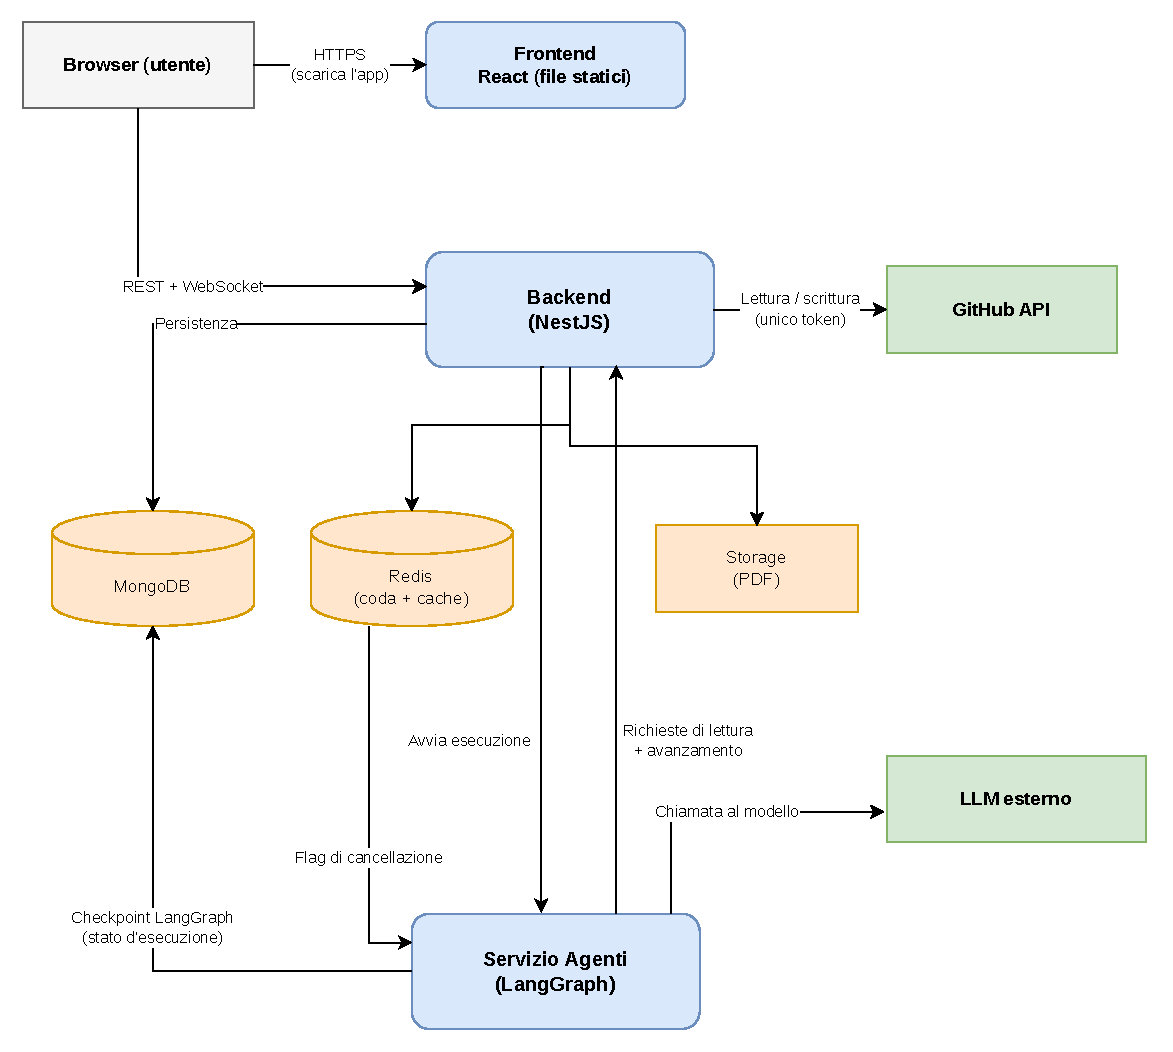
\includegraphics[width=0.95\textwidth]{vista-insieme.pdf}
    \caption{Vista d'insieme dei servizi di Code Guardian e dei loro collegamenti.}
    \label{fig:vista-insieme}
\end{figure}

Dal punto di vista dell'utente il sistema espone un'unica origine web. Il browser scarica il Frontend, un'applicazione React compilata in file statici, e da quel momento parla solo con il Backend: chiamate REST da un lato, un canale \textit{\glo{WebSocket}{websocket}} dedicato agli aggiornamenti in tempo reale delle operazioni in corso dall'altro. Frontend e Backend restano comunque due unità distinte, e aggiornare l'una non richiede di ridistribuire l'altra: il loro unico punto di contatto è il contratto REST/WebSocket.

Il Backend è il fulcro del sistema. È l'unico componente che detiene le credenziali dell'utente, inclusa quella verso GitHub, che resta cifrata; l'unico che persiste i dati applicativi, cioè utenti, credenziali, contesti di analisi, Task e Report; e l'unico autorizzato a modificare i repository sorvegliati, tramite l'apertura automatica di Pull Request. Riceve le richieste dal Frontend, le traduce in unità di lavoro (le Task) e ne affida l'esecuzione al servizio Agenti. Resta poi suo il compito di raccogliere l'esito, persisterlo e notificarlo all'utente.

%%%% DA VERIFICARE E SISTEMARE CON IL GRUPPO - non siamo sicuri se tenerlo cosi' o meno %%%%
Il servizio Agenti condivide con il Backend la stessa istanza di MongoDB e la stessa istanza di Redis, ma con un ruolo molto più circoscritto: vi legge e scrive soltanto lo stato interno delle proprie esecuzioni, cioè il punto da cui un'analisi sospesa può riprendere in un secondo momento e un'eventuale richiesta di annullamento in corso. Nessun dato applicativo di dominio, quindi: né Task, né Report, né credenziali.

Il servizio Agenti resta invece isolato dal resto del sistema, per scelta. È l'unico a dialogare con il modello linguistico (LLM), ma non ha credenziali verso GitHub e non può raggiungere Internet: quando un agente deve leggere un file di un repository o l'elenco delle sue issue, chiede quel contenuto al Backend, che lo recupera per suo conto. Il token dell'utente resta così confinato in un solo servizio, e si riduce la superficie d'attacco del componente più esposto all'imprevedibilità di un modello linguistico. Anche nella peggiore delle ipotesi, un agente compromesso non avrebbe un canale attraverso cui uscire.

La comunicazione tra Backend e Agenti è quindi bidirezionale, ma asimmetrica nei permessi. Il Backend avvia l'esecuzione di un agente e ne riceve il risultato finale; l'agente, mentre lavora, può solo richiedere al Backend le singole letture di cui ha bisogno. Nessuna delle due direzioni espone un endpoint pubblico: è traffico interno, non raggiungibile né dal Frontend né da Internet.

L'esecuzione di un'operazione è disaccoppiata dalla richiesta dell'utente. Il Backend accoda il lavoro e risponde subito; l'esecuzione effettiva avviene in background e l'esito raggiunge il Frontend attraverso il canale realtime. I dettagli di questo meccanismo arrivano più avanti. In questa vista d'insieme conta un punto solo: nessun worker resta bloccato ad attendere la risposta lenta di un'altra unità o un intervento umano, perché il lavoro in corso viene checkpointato e il worker che lo eseguiva torna subito disponibile.

\subsection{Architettura di Deployment}
\label{subsec:deployment}

La vista d'insieme descrive chi parla con chi; qui si vede dove ciascun componente gira fisicamente e attraverso quali confini di rete passa ogni collegamento. L'infrastruttura di produzione è ospitata su AWS, all'interno di un'unica rete privata virtuale (\textit{\glo{VPC}{vpc}}) distribuita su due \textit{Availability Zone}, il minimo tecnico richiesto per poter attivare un Application Load Balancer. Come emerge più avanti in questa stessa sezione, i singoli servizi restano a istanza unica: la topologia multi-AZ è più una predisposizione di rete che una protezione attiva contro un guasto.

\begin{figure}[H]
    \centering
    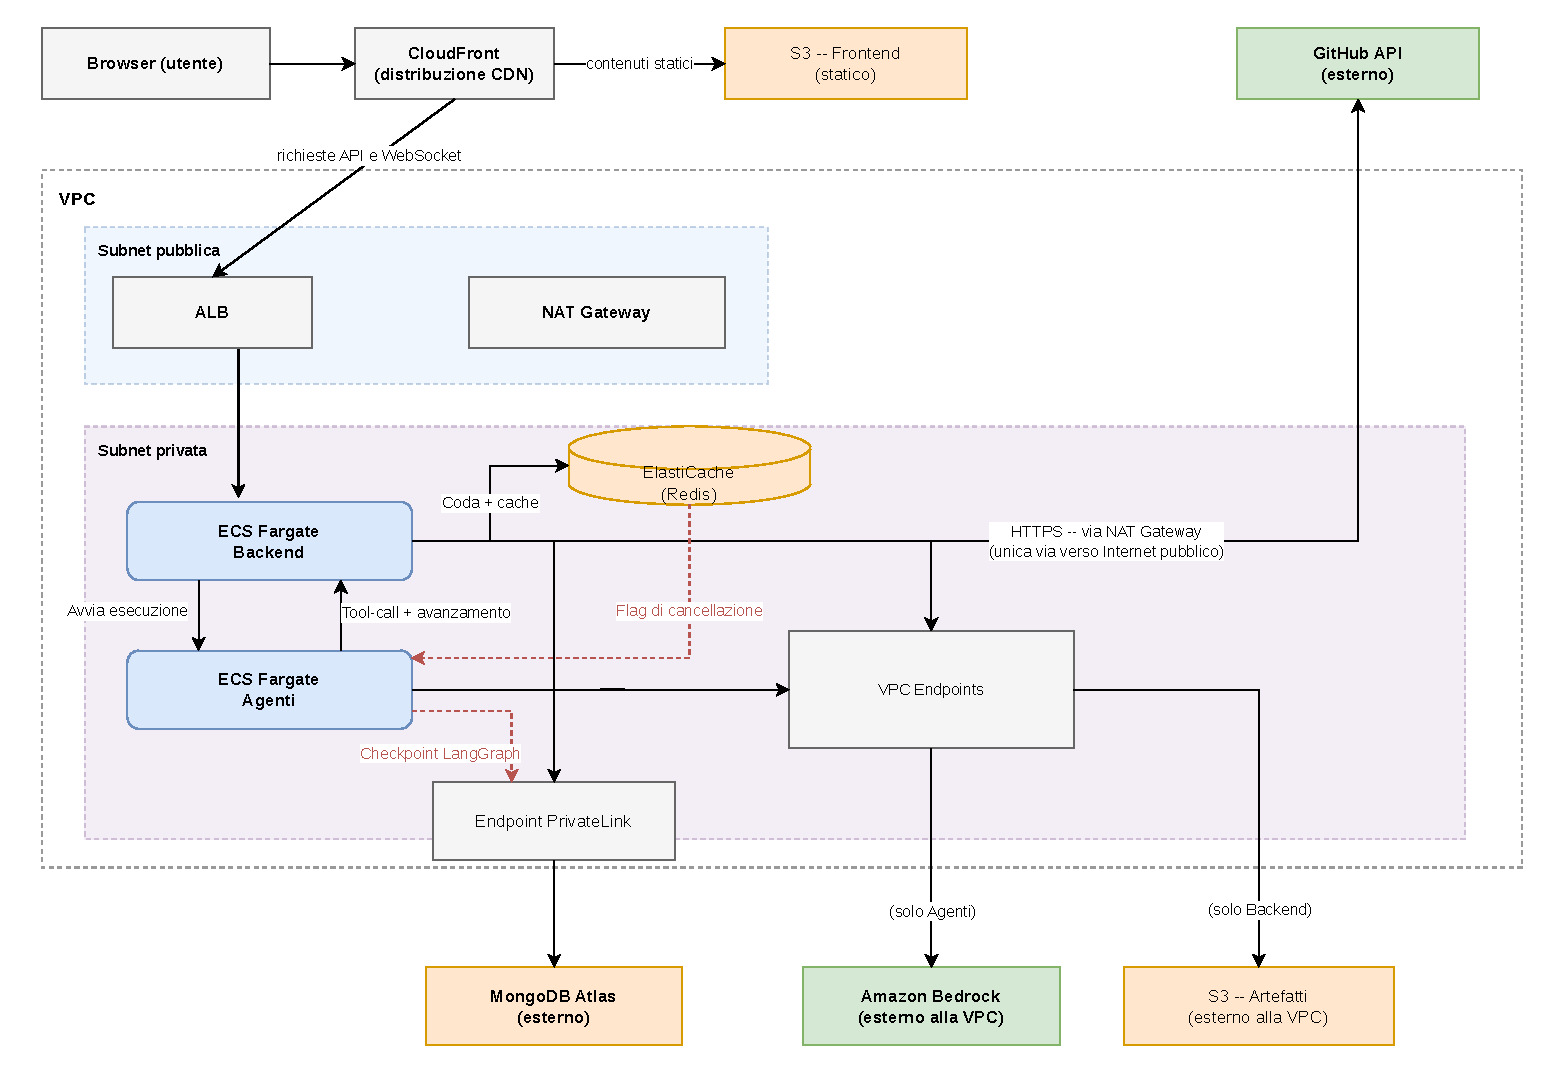
\includegraphics[width=0.95\textwidth]{architettura-deployment.pdf}
    \caption{Architettura di deployment su AWS.}
    \label{fig:deployment}
\end{figure}

La VPC è divisa in subnet pubbliche e private. Solo le prime raggiungono direttamente Internet; le subnet private instradano il traffico in uscita attraverso un unico \textit{\glo{NAT Gateway}{nat-gateway}}. Backend e Agenti girano entrambi in subnet private dello stesso tipo, quindi a limitare concretamente l'accesso a Internet del servizio Agenti non è la subnet in cui si trova, ma il suo Security Group, configurato secondo un principio di \emph{default deny}: il traffico in uscita è permesso solo verso destinazioni esplicitamente elencate. Ogni componente ha un proprio Security Group dedicato, e ciascuno nega per difetto tutto il traffico non concesso.

Il percorso pubblico non cambia rispetto alla vista d'insieme: un'unica distribuzione CloudFront riceve tutto il traffico del browser e lo instrada verso due origini diverse a seconda del percorso richiesto, i file statici del Frontend, letti da un bucket S3 privato, oppure il Backend, raggiunto attraverso un Application Load Balancer (ALB). L'ALB non possiede un proprio certificato \textit{\glo{TLS}{tls}}. È CloudFront a terminare HTTPS verso il browser, mentre il collegamento tra CloudFront e l'ALB resta in HTTP semplice, comunque confinato all'interno della rete di AWS. Il bucket del Frontend resta privato, leggibile solo da CloudFront tramite un meccanismo dedicato (\textit{Origin Access Control}). CloudFront restituisce inoltre la pagina applicativa sui percorsi non gestiti dal bucket, così che il routing lato client funzioni anche dopo un ricaricamento diretto della pagina.

Backend e Agenti sono due servizi ECS su Fargate distinti, ciascuno con il proprio dimensionamento di CPU e memoria, proporzionato al carico atteso: il servizio Agenti riceve più risorse, essendo quello che dialoga con il modello linguistico. Entrambi girano oggi con una singola replica: una semplificazione che abbiamo accettato per l'MVP. Per compensare l'assenza di ridondanza, ogni distribuzione richiede che la nuova versione sia effettivamente in salute prima di terminare quella precedente, e viene annullata automaticamente se la nuova versione non ci arriva mai.

Entrambi i servizi girano come processi a lunga vita, e non come funzioni invocate una tantum per singola richiesta: un modello di esecuzione puramente serverless non potrebbe sostenere un worker che consuma di continuo una coda, né una connessione WebSocket aperta per l'intera durata di una Task. La sospensione di un'esecuzione, quando avviene, non richiede comunque che il processo resti vivo ad attenderla. Lo stato viene esternalizzato come checkpoint su MongoDB (\S~\ref{subsec:agenti}) e il worker che l'ha gestita torna subito disponibile. A imporre due servizi containerizzati sempre attivi, invece di un modello \textit{serverless}, sono quindi il worker e il canale realtime, non lo stato sospeso.

A runtime Backend e Agenti si trovano tramite una zona DNS privata interna, già introdotta nella vista d'insieme e non raggiungibile dall'esterno della rete: ciascun servizio si registra con un nome stabile, e l'altro lo risolve senza che nessuno dei due debba conoscere in anticipo un indirizzo IP.

Il livello dati vive anch'esso interamente all'interno della rete privata. MongoDB è ospitato su MongoDB Atlas, un servizio gestito esterno ad AWS: il progetto prevede di raggiungerlo attraverso un collegamento privato dedicato (PrivateLink) invece che tramite Internet pubblico, così che il cluster non debba accettare connessioni dalla rete pubblica. Redis (ElastiCache) gira invece come singola istanza: un altro rischio che abbiamo accettato per l'MVP.

Oltre a queste due destinazioni, la rete privata include una serie di collegamenti dedicati verso gli altri servizi AWS di cui Backend e Agenti hanno bisogno, dalla gestione dei segreti al registro delle immagini container. Quel traffico non esce così dalla rete privata e non passa dal NAT Gateway. Il collegamento verso il modello linguistico (Amazon Bedrock) è uno di questi, con una particolarità: è raggiungibile soltanto dal Security Group del servizio Agenti. Il vincolo per cui solo l'Agente può invocare il modello vale quindi anche a livello di rete, non solo nel codice applicativo.

Rimane infine il canale principale che attraversa il confine della rete privata verso l'Internet pubblico: quello del Backend verso l'API di GitHub, instradato attraverso il NAT Gateway.

\subsection{Architettura del Frontend}
\label{subsec:frontend}

Il Frontend è un'applicazione a pagina singola (\textit{Single-Page Application}): una volta caricata, il browser non richiede più pagine intere al server e sostituisce il contenuto a schermo interamente lato client. Anche l'instradamento tra le schermate (\textit{routing}) avviene quindi nel browser, ed è possibile grazie all'origine unica descritta in §3.2. Senza la riscrittura degli errori operata da CloudFront, un accesso diretto o un ricaricamento su un percorso profondo dell'applicazione non funzionerebbe.

Le rotte sono divise in due gruppi: un piccolo insieme di rotte pubbliche (accesso, registrazione) e un gruppo di rotte autenticate (configurazione delle credenziali, selezione del contesto, avvio delle operazioni, dashboard, storico e dettaglio dei report), annidate sotto un'unica intestazione applicativa condivisa. Prima di mostrare una schermata autenticata il router verifica sincronamente lo stato di sessione già presente in memoria: nessuna attesa di rete, navigazione istantanea.

Lo stato applicativo condiviso è diviso in tre store distinti, ciascuno responsabile di un solo dominio: l'identità e la sessione dell'utente, il contesto operativo scelto in fase di configurazione, e lo stato in tempo reale delle operazioni in corso. Tutto ciò che non deve sopravvivere a un cambio di rotta, né essere letto da più componenti insieme, resta nello stato locale della singola schermata che lo usa.

\begin{figure}[H]
    \centering
    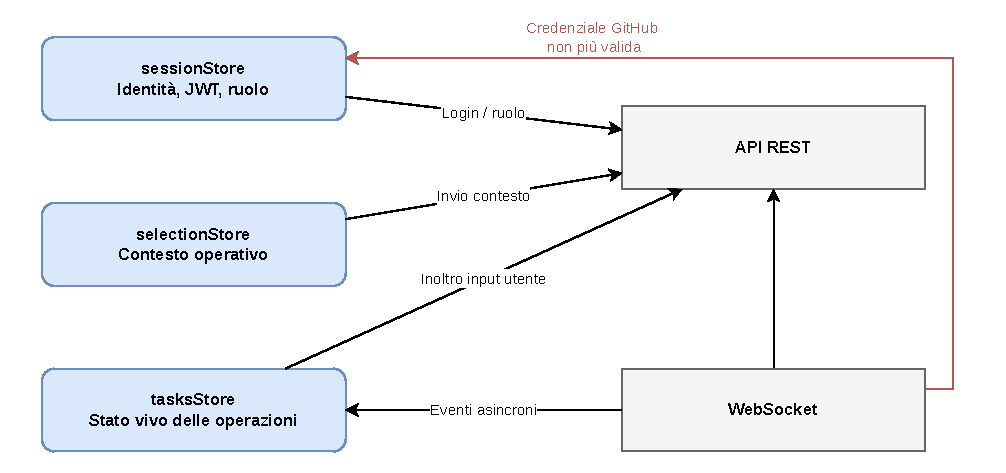
\includegraphics[width=0.9\textwidth]{frontend-stores.pdf}
    \caption{Architettura degli store applicativi e comunicazione di rete.}
    \label{fig:frontend-stores}
\end{figure}

Lo store dedicato alle operazioni non riceve i propri dati soltanto dal canale WebSocket già descritto in §3.1; viene scritto anche da chiamate REST dirette — al caricamento iniziale della schermata e per riflettere localmente un annullamento richiesto dall'utente. Il canale WebSocket resta comunque la fonte primaria degli aggiornamenti di stato durante l'esecuzione di un'operazione. Poiché quel canale non garantisce la consegna degli eventi emessi durante un'eventuale disconnessione, alla riconnessione il Frontend richiede nuovamente lo stato delle operazioni tramite API REST.

Un solo caso vede un singolo evento aggiornare due store anziché uno: quando il canale realtime segnala che le credenziali configurate non sono più valide, lo stesso evento tocca sia lo stato delle operazioni sia lo stato di sessione, attivando insieme l'avviso persistente in interfaccia e le guardie di rotta. I due store restano comunque indipendenti: nessuno dei due richiama l'altro, è l'evento a raggiungere entrambi.

Il token di sessione (JWT) resta in memoria e non tocca lo storage persistente del browser: un ricaricamento completo della pagina invalida quindi la sessione corrente e richiede un nuovo accesso. Abbiamo accettato il compromesso per ridurre la superficie di attacco, in un perimetro che per l'MVP non prevede protezioni avanzate contro script malevoli lato client.

Verso il Backend il Frontend usa solo percorsi relativi sotto un unico prefisso, senza domini assoluti. Il Backend riceve la propria configurazione a runtime; il Frontend invece è distribuito come artefatto statico già compilato, e un indirizzo assoluto cablato al suo interno resterebbe fissato in modo irreversibile per ogni ambiente in cui quello stesso pacchetto venisse distribuito. Lo stesso token di sessione autentica sia le chiamate REST sia l'apertura del canale WebSocket.

La gestione degli errori distingue due famiglie, con pattern d'interfaccia diversi. Gli errori di validazione e configurazione sono sincroni: l'utente li risolve subito, senza lasciare la schermata corrente, e compaiono in prossimità del campo interessato. Gli errori di esecuzione di un'operazione sono invece asincroni, emergono a distanza di tempo dall'avvio tramite il canale realtime, e passano da un unico componente condiviso, alimentato da un catalogo chiuso di codici d'errore chiuso lato Backend.

\subsection{Architettura del Backend}
\label{subsec:backend}

Come anticipato nella vista d'insieme, il Backend è organizzato per dominio funzionale più che per livello tecnico: non esistono cartelle trasversali condivise da tutto il progetto, ma un modulo NestJS autonomo per ciascuna area di competenza (identità, credenziali, integrazione GitHub, contesti di analisi, task, operazioni, report, comunicazione realtime), ciascuno con i propri controller, servizi e schema di persistenza. È l'organizzazione idiomatica suggerita dallo stesso framework, e lascia lavorare in parallelo su moduli diversi senza sovrapposizioni.

Le due sottosezioni seguenti approfondiscono le aree del Backend con la struttura interna più articolata: l'integrazione con GitHub e l'orchestrazione dell'esecuzione delle Task. Le restanti responsabilità, come l'autenticazione, la cifratura delle credenziali e la validazione del contesto di analisi, seguono lo stesso principio di organizzazione, con una struttura interna troppo semplice per giustificare un diagramma dedicato.

\subsubsection{Integrazione con GitHub}

Nessun componente diverso dal Backend detiene il token GitHub dell'utente, né lo espone all'esterno. È il confine più importante dell'intero sistema, e regge su due percorsi separati e asimmetrici: uno di sola lettura, esposto agli agenti attraverso una facade interna, e uno di scrittura, riservato al solo Backend.

\begin{figure}[H]
    \centering
    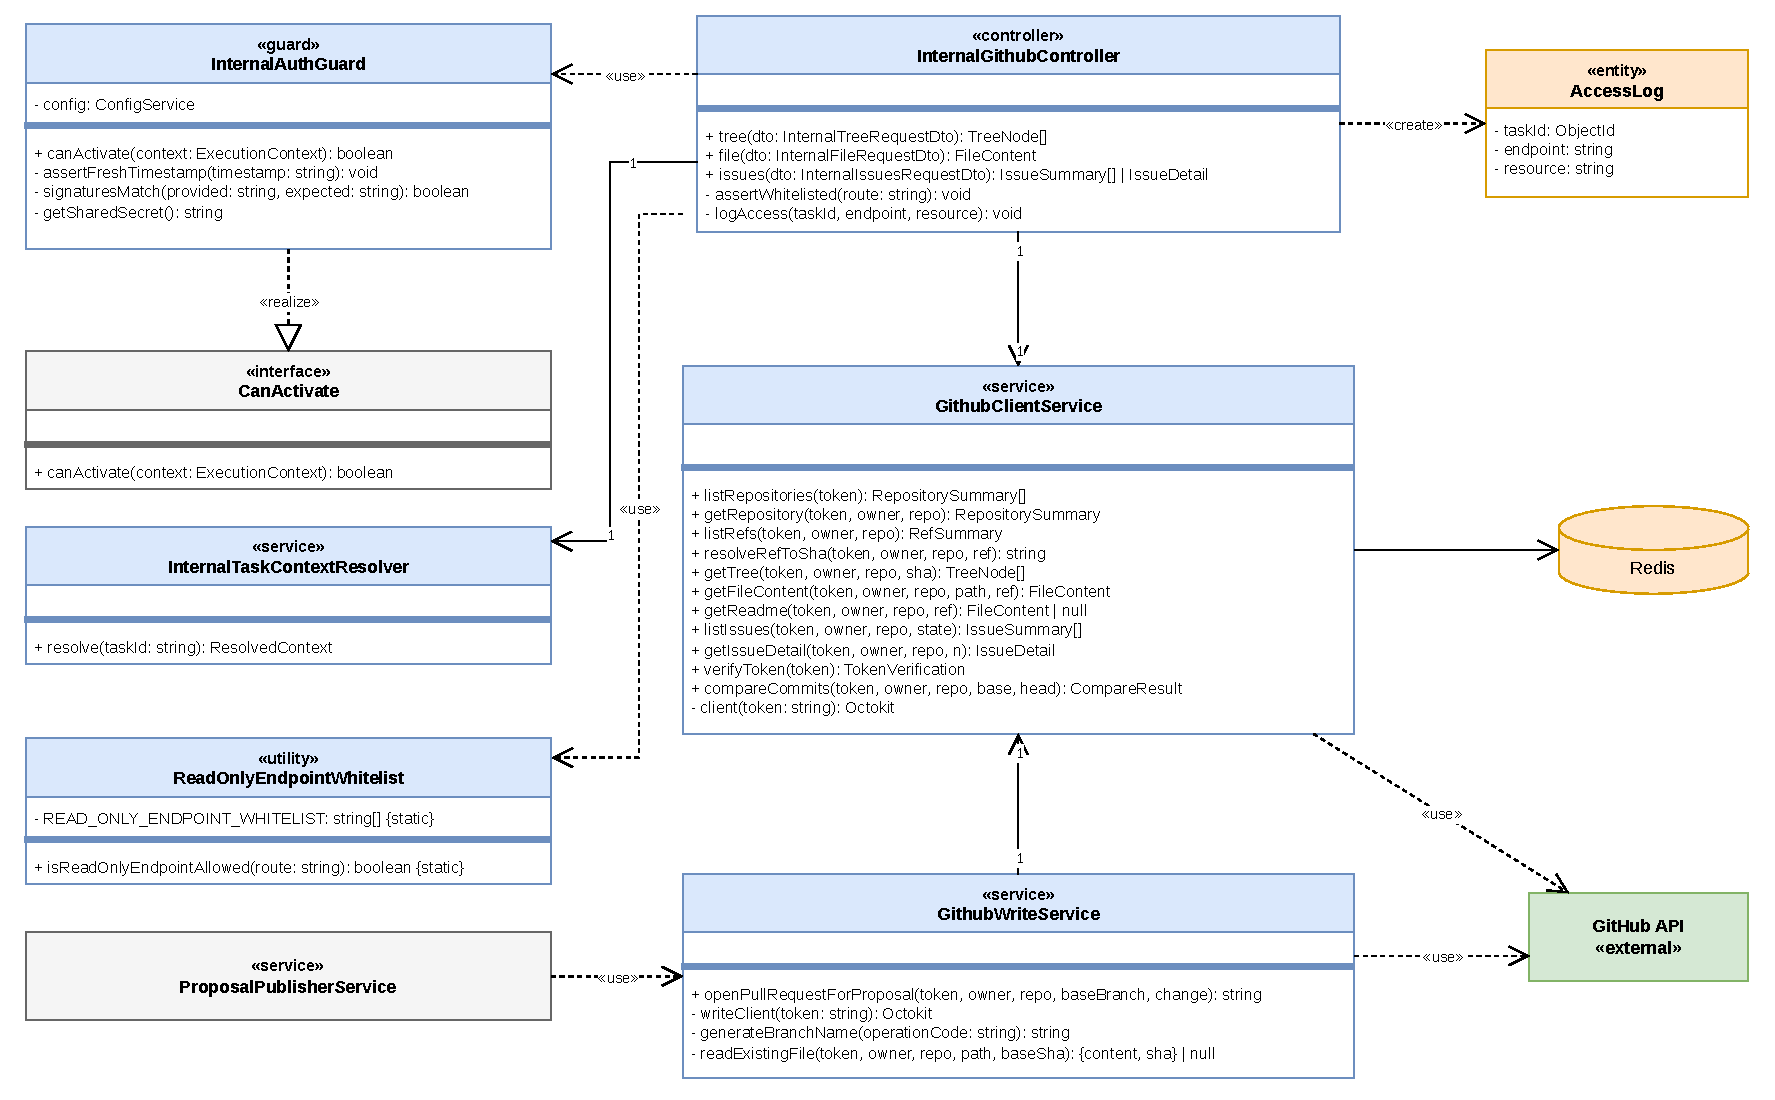
\includegraphics[width=0.95\textwidth]{backend-github-integration.pdf}
    \caption{Struttura interna dell'integrazione con GitHub.}
    \label{fig:backend-github}
\end{figure}

Il percorso di lettura è \texttt{InternalGithubController}: un endpoint interno, non documentato pubblicamente e raggiungibile solo dalla rete privata, protetto da una firma \textit{\glo{HMAC}{hmac}} verificata da \texttt{InternalAuthGuard} anziché da un token utente, poiché il chiamante è un servizio e non una persona. Ogni chiamata attraversa tre controlli prima di raggiungere GitHub. Viene innanzitutto verificata contro un elenco chiuso di operazioni permesse, costruito sugli stessi identificativi di rotta usati dal client GitHub reale, in modo che quell'elenco e le chiamate effettive non possano divergere. Il contesto (repository, commit, token dell'utente) viene poi risolto a partire dal solo identificativo della Task. L'accesso viene infine registrato come riga di \texttt{AccessLog}, così il vincolo di sola lettura resta verificabile a posteriori. Le chiamate effettive verso GitHub passano tutte da \texttt{GithubClientService}, che rifiuta per costruzione qualunque richiesta che non sia una \texttt{GET}.

Redis, oltre a fare da coda per l'esecuzione asincrona, compare qui anche come cache delle letture più ripetute nel corso di un'analisi: la struttura del repository, il contenuto dei singoli file e il README. La cache è indicizzata per repository e per commit; poiché il contenuto di un repository a un commit specifico è per definizione immutabile, un dato già in cache non può risultare obsoleto. Si riduce così la pressione sulla quota dell'API di GitHub, condivisa da tutte le richieste del sistema.

Il percorso di scrittura vive in una classe a sé, \texttt{GithubWriteService}, per non indebolire quella garanzia. Riusa \texttt{GithubClientService} solo per le proprie letture di supporto, ad esempio risolvere un branch o leggere il contenuto attuale di un file, mentre apre branch, commit e Pull Request con un proprio client. Nessun agente vi ha accesso: a invocarlo, soltanto dopo che un agente ha già terminato la propria esecuzione, è \texttt{ProposalPublisherService}, descritto nel dettaglio nella sezione successiva.
\subsubsection{Orchestrazione ed Esecuzione}

A decidere verso quale agente instradare un'operazione è una tabella statica, non il modello linguistico: \texttt{AgentRegistry} associa ogni codice operazione al proprio agente, ai ruoli abilitati a richiederlo e al tempo massimo concesso per l'esecuzione. La stessa tabella filtra il catalogo delle operazioni mostrato all'utente e i controlli di autorizzazione all'avvio di una Task.

\begin{figure}[H]
    \centering
    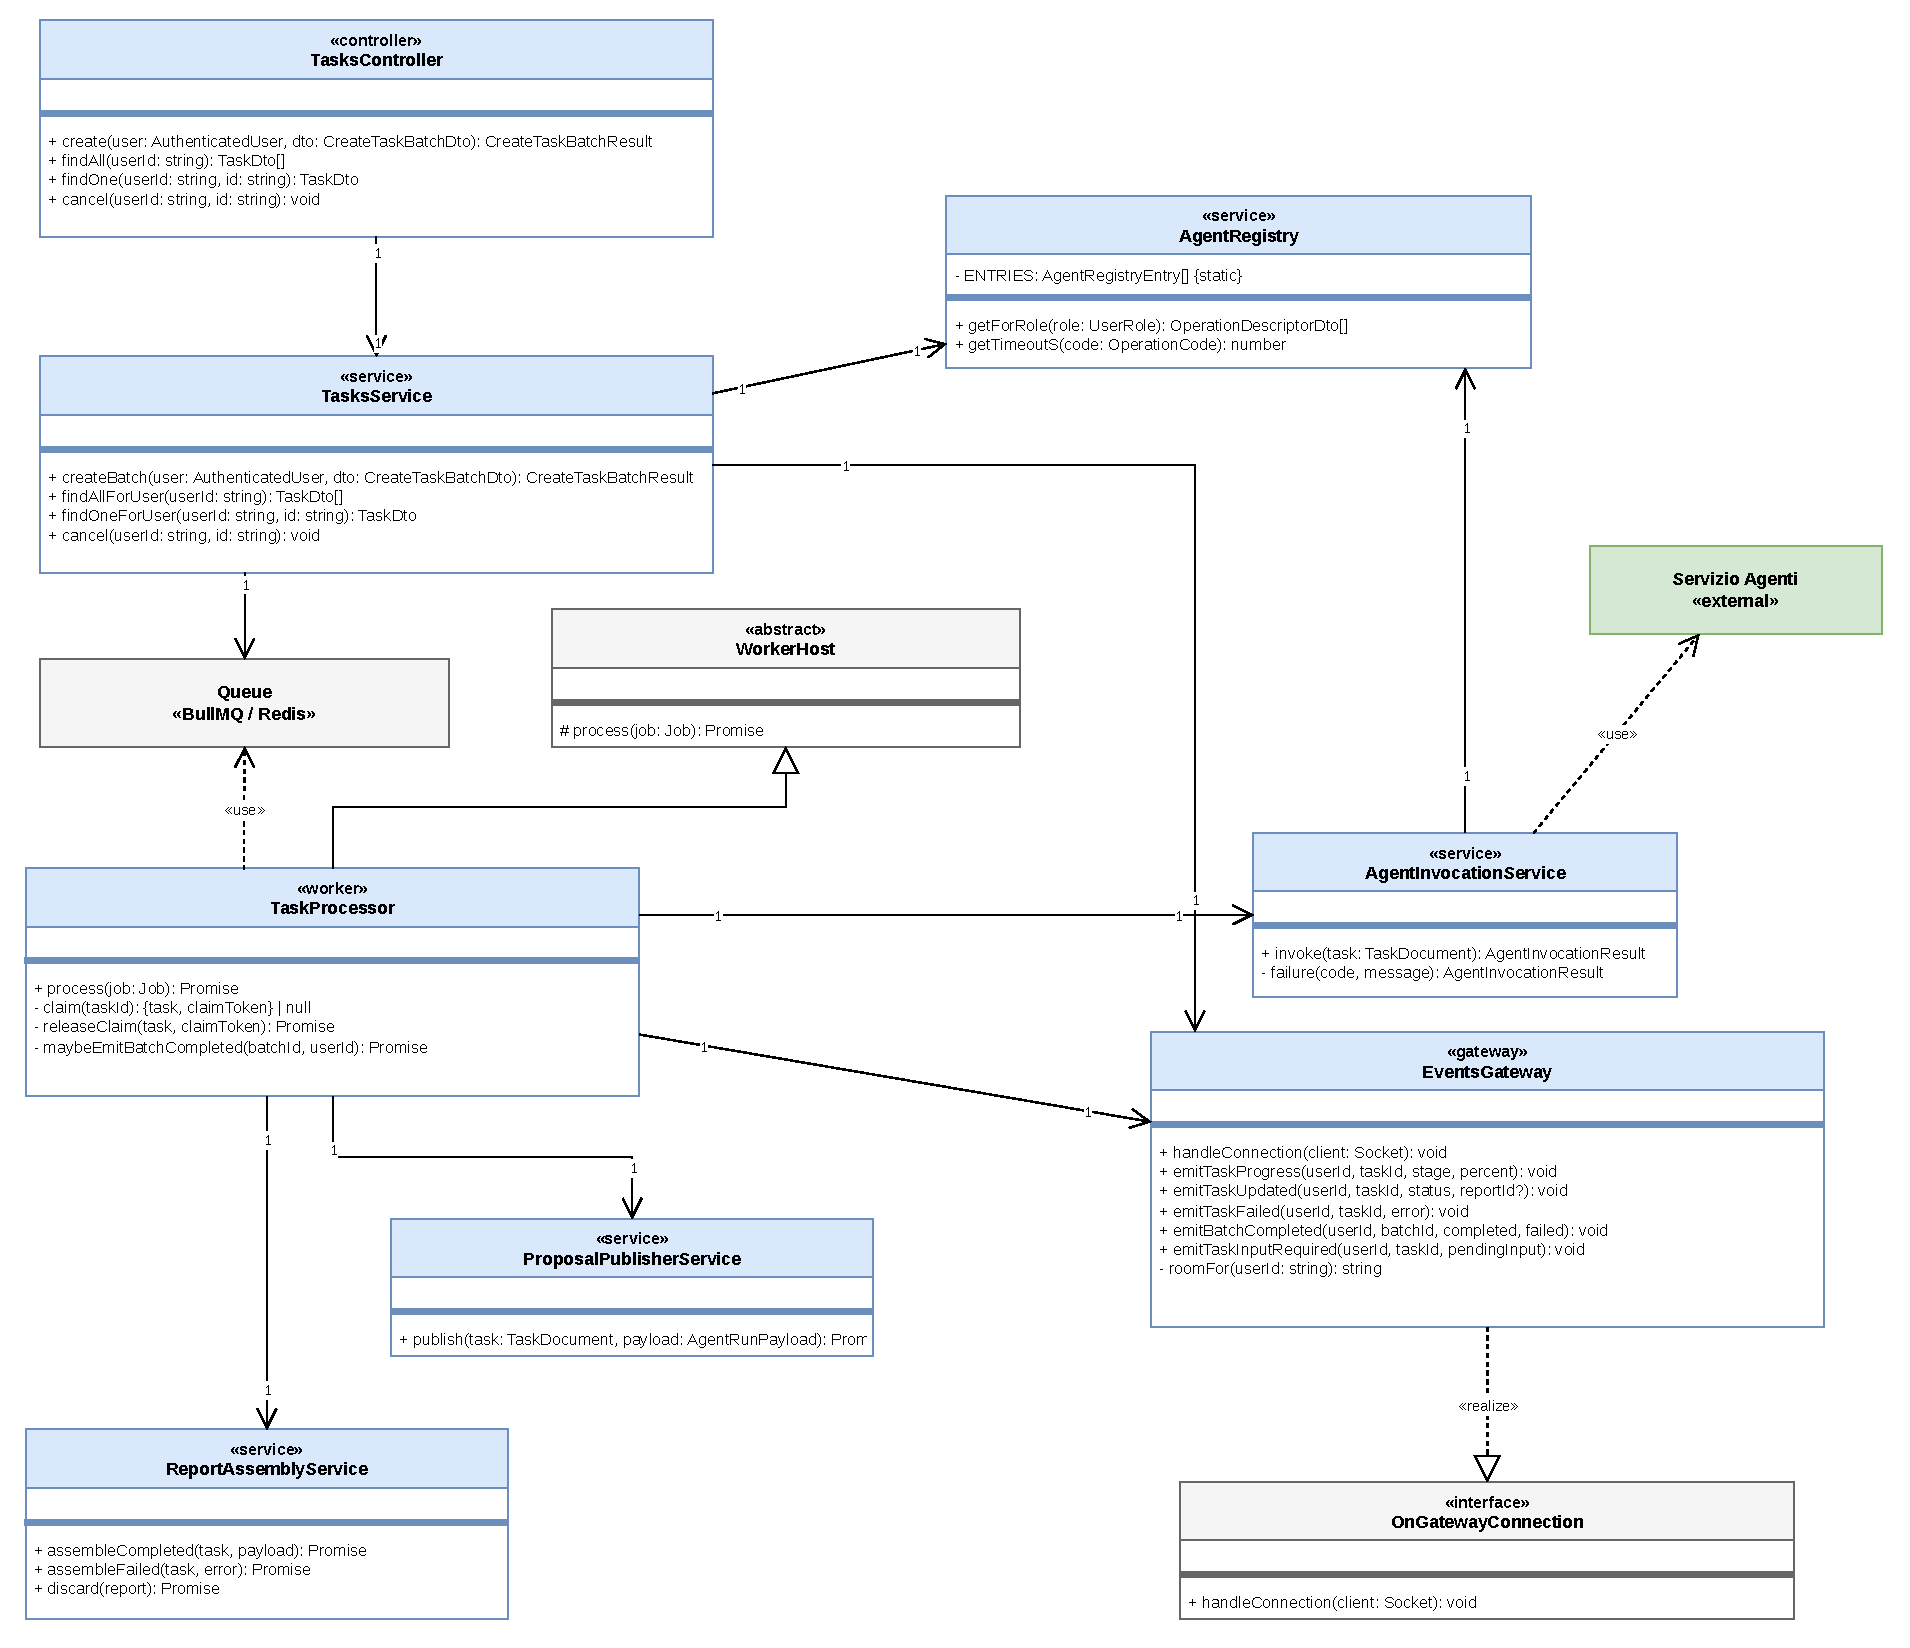
\includegraphics[width=0.95\textwidth]{backend-task-orchestration.pdf}
    \caption{Struttura interna dell'orchestrazione ed esecuzione delle Task.}
    \label{fig:backend-orchestration}
\end{figure}

\texttt{TasksController} e \texttt{TasksService} gestiscono il ciclo di vita di una Task dalla richiesta alla persistenza, ma non la eseguono. L'avvio di un batch si conclude accodando un job per ciascuna Task, e la richiesta HTTP termina subito. A prelevare i job uno alla volta e a invocare l'agente tramite \texttt{AgentInvocationService} è \texttt{TaskProcessor}, un consumatore della coda separato dal ciclo della richiesta. Un job che fallisce aggiorna solo la propria Task e non tocca le altre in coda. Ogni cambiamento di stato, sia esso di avanzamento, completamento o fallimento, viene propagato al Frontend da \texttt{EventsGateway} sul canale WebSocket già descritto in precedenza: la distribuzione avviene per utente e non per singola Task, quindi basta un'unica connessione per tenere aggiornata la dashboard su più operazioni in corso contemporaneamente.

Il risultato di un agente completato non raggiunge il Frontend direttamente, attraversa prima \texttt{ProposalPublisherService} che apre la Pull Request quando l'agente ha prodotto una Proposal. Solo dopo \texttt{ReportAssemblyService} costruisce il Report vero e proprio a partire da quel payload. È soltanto a valle di questi due passaggi che \texttt{TaskProcessor} invoca \texttt{EventsGateway} per notificare l'esito al Frontend.
Il meccanismo di sospensione e ripresa di un'esecuzione, e il protocollo dettagliato tra Backend e Agenti, sono discussi più avanti in questo documento.

\subsubsection{Il contratto Report}

Qualunque sia l'agente che l'ha prodotto, il Backend persiste ed espone sempre lo stesso tipo di oggetto: un \texttt{Report}, con un'intestazione fissa e un corpo composto da un elenco di blocchi polimorfi. Il contratto è unico e condiviso, non specializzato per singolo agente: Backend e Frontend trattano il risultato di un'analisi senza sapere quale dei tre agenti lo abbia generato.

\begin{figure}[H]
    \centering
    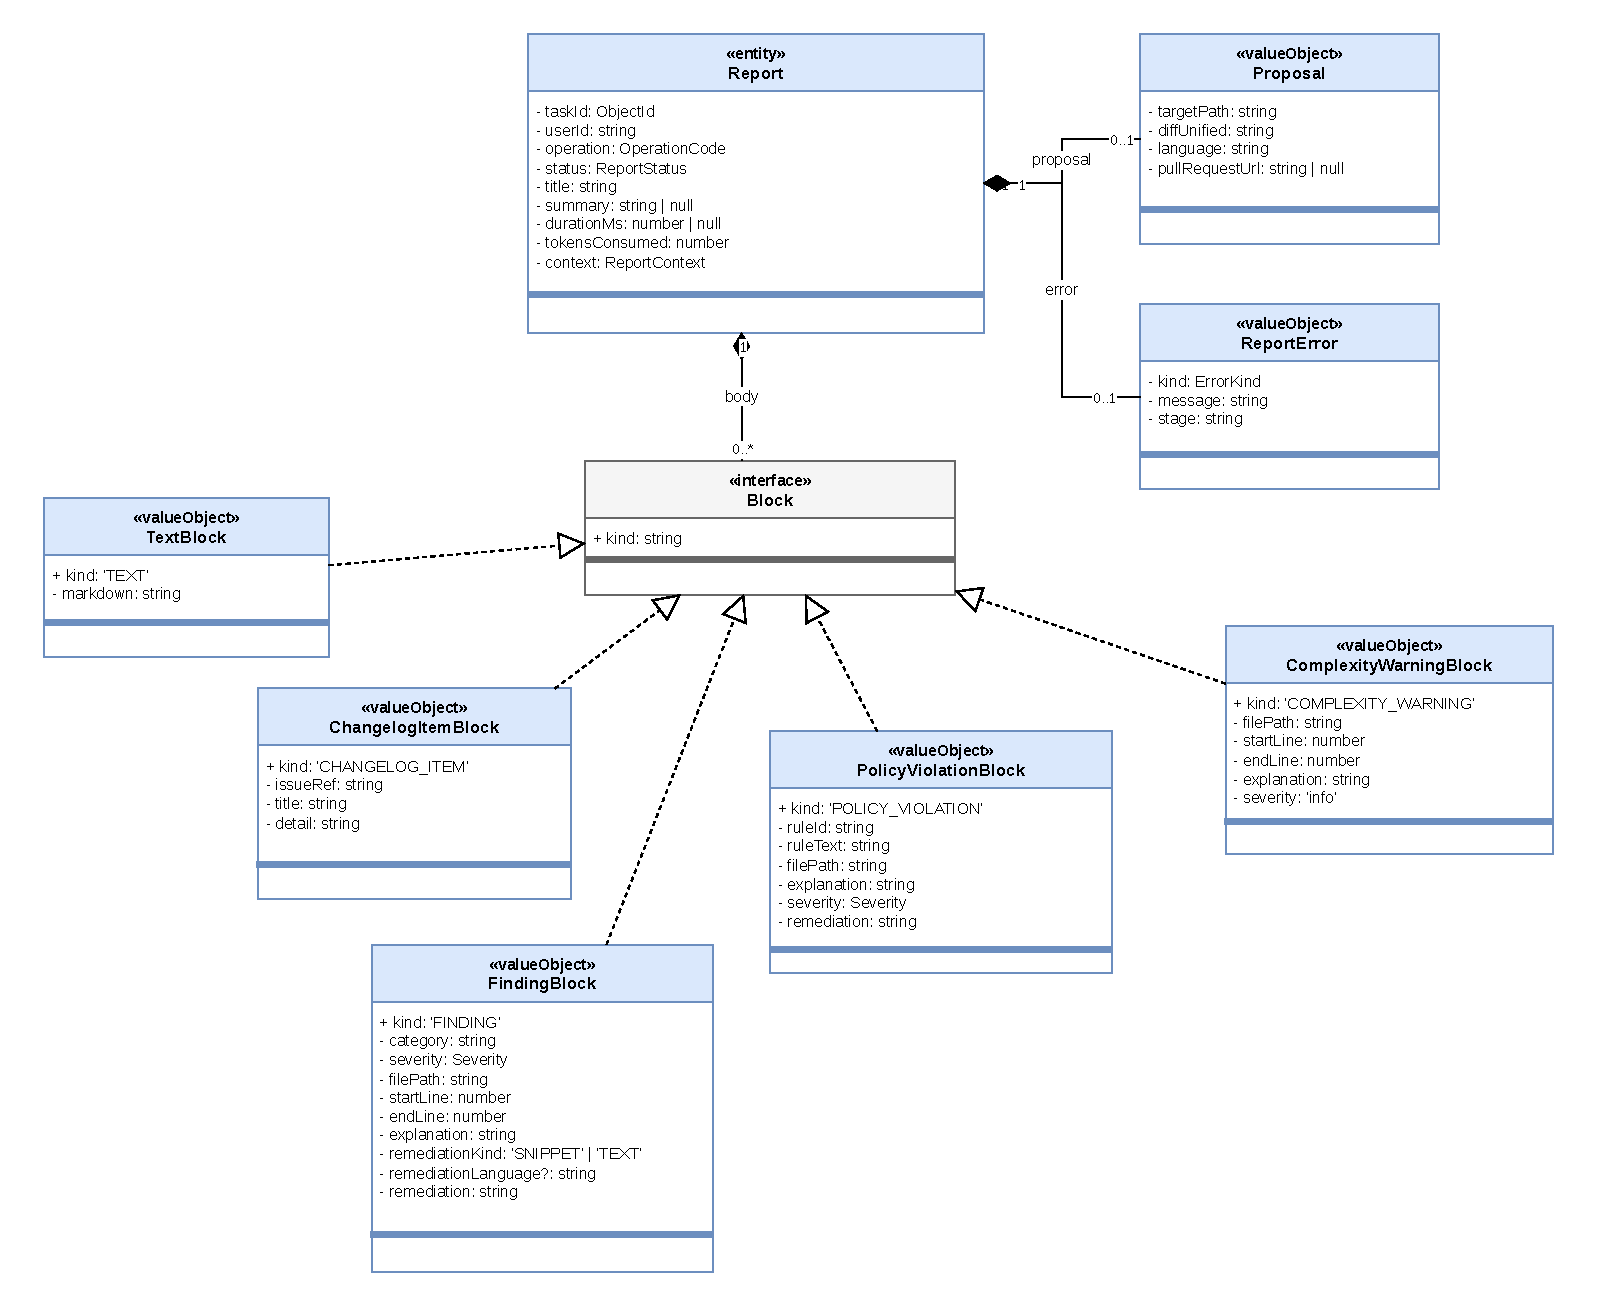
\includegraphics[width=0.95\textwidth]{backend-report-blocks.pdf}
    \caption{Struttura del Report}
    \label{fig:backend-report-blocks}
\end{figure}

Ogni agente riempie il corpo del Report in modo diverso: l'Agente Docs produce soprattutto una \texttt{Proposal}, cioè un diff verso il file di destinazione; l'Agente Security riempie una lista di \texttt{FindingBlock} o \texttt{PolicyViolationBlock} a seconda dell'operazione, con eventuali \texttt{ComplexityWarningBlock} e, per la sola scansione OWASP, i \texttt{SastFindingBlock} e il \texttt{SastSummaryBlock} prodotti dall'integrazione Semgrep; l'Agente Changelog produce uno o più \texttt{TextBlock} o \texttt{ChangelogItemBlock}. Un campo \texttt{order} numerico, presente su ogni tipo di blocco, ne fissa l'ordine di visualizzazione. Nessuno di questi tipi introduce un percorso di codice separato nel Backend. La persistenza, l'esposizione via API e l'esportazione in PDF trattano il corpo del Report come un array indifferenziato, e l'interpretazione del contenuto resta a chi lo consuma.
\subsubsection{Gestione degli Errori}

Un'analisi può fallire per ragioni molto diverse tra loro (un timeout del modello linguistico, un token GitHub non più valido, un limite di utilizzo superato), ma il sistema le riconduce tutte a un vocabolario chiuso di codici. Non è però un'unica definizione condivisa tra i due linguaggi: il Servizio Agenti dichiara il proprio \texttt{ErrorKind} in Python, il Backend il proprio in TypeScript. Il catalogo del Backend è un soprainsieme perché include codici che l'agente non produce mai che nascono da fallimenti propri del Backend. Un errore che nasce lato agente viene tradotto nel corrispondente codice del Backend mentre attraversa il confine tra i due servizi. Un codice che il Backend non riconosce non viene propagato così com'è: viene ricondotto a un valore generico \texttt{UPSTREAM}.

Un normalizzatore centralizzato sul Backend traduce ogni errore in una risposta HTTP di forma identica (un codice, un messaggio, eventuali dettagli di validazione) prima che raggiunga il Frontend. La stessa convenzione sui codici vale anche sul canale asincrono: un errore emerso a metà di una Task raggiunge il Frontend con lo stesso codice di una risposta REST. L'involucro che lo trasporta resta però diverso, un oggetto annidato sotto \texttt{error} invece della forma piatta REST. \texttt{CREDENTIAL\_INVALID} ne è un esempio concreto: lo stesso codice viene riconosciuto sia quando GitHub rifiuta un token al salvataggio, sia quando quel token si rileva non funzionante a metà di una operazione già avviata, e in entrambi i casi compare lo stesso avviso con reindirizzamento alla schermata delle credenziali.

\subsection{Architettura del Servizio Agenti}
\label{subsec:agenti}

Il Servizio Agenti è un processo Python separato (FastAPI), responsabile della sola parte del sistema che ragiona: comporre un prompt, invocare il modello linguistico, ed eventualmente correggere o completare il proprio output prima di restituirlo. Comunica con il Backend soltanto attraverso i due endpoint interni già introdotti, \texttt{/internal/agent/start} e \texttt{/internal/agent/resume}. Ogni chiamata è sincrona, e la risposta contiene o il risultato completo, o il motivo per cui l'esecuzione si è interrotta. Il servizio non scrive mai direttamente su GitHub e non sceglie da sé quale credenziale usare: entrambe le responsabilità restano dove il Backend le ha collocate.

\subsubsection{Un solo scheletro, tre configurazioni}

\texttt{AgentGraph} è un unico grafo di esecuzione parametrizzato su tre punti di estensione, e i tre agenti ne sono tre configurazioni diverse: la logica di orchestrazione è scritta una volta sola. Un \texttt{Loader} è l'adattatore che, prima ancora di comporre un prompt, recupera dal repository (attraverso la stessa facade GitHub) il materiale grezzo su cui l'agente dovrà ragionare: per gli agenti Docs e Changelog carica per intero ciò che serve, rispettivamente l'albero e il contenuto dei file nell'ambito scelto, o le issue chiuse dello sprint; per l'Agente Security carica solo l'albero del repository, lasciando che sia il modello stesso a chiedere, un file alla volta, il contenuto di ciò che ritiene rilevante. Un \texttt{Profile} sa come trasformare quel materiale in un prompt e come interpretare la risposta del modello, producendo i blocchi del Report. Un \texttt{LLMProvider}, infine, sa come invocare concretamente il modello al provider Amazon Bedrock. Cambiare agente significa sostituire la coppia Loader/Profile, non riscrivere il modo in cui il grafo viene eseguito.

\begin{figure}[H]
    \centering
    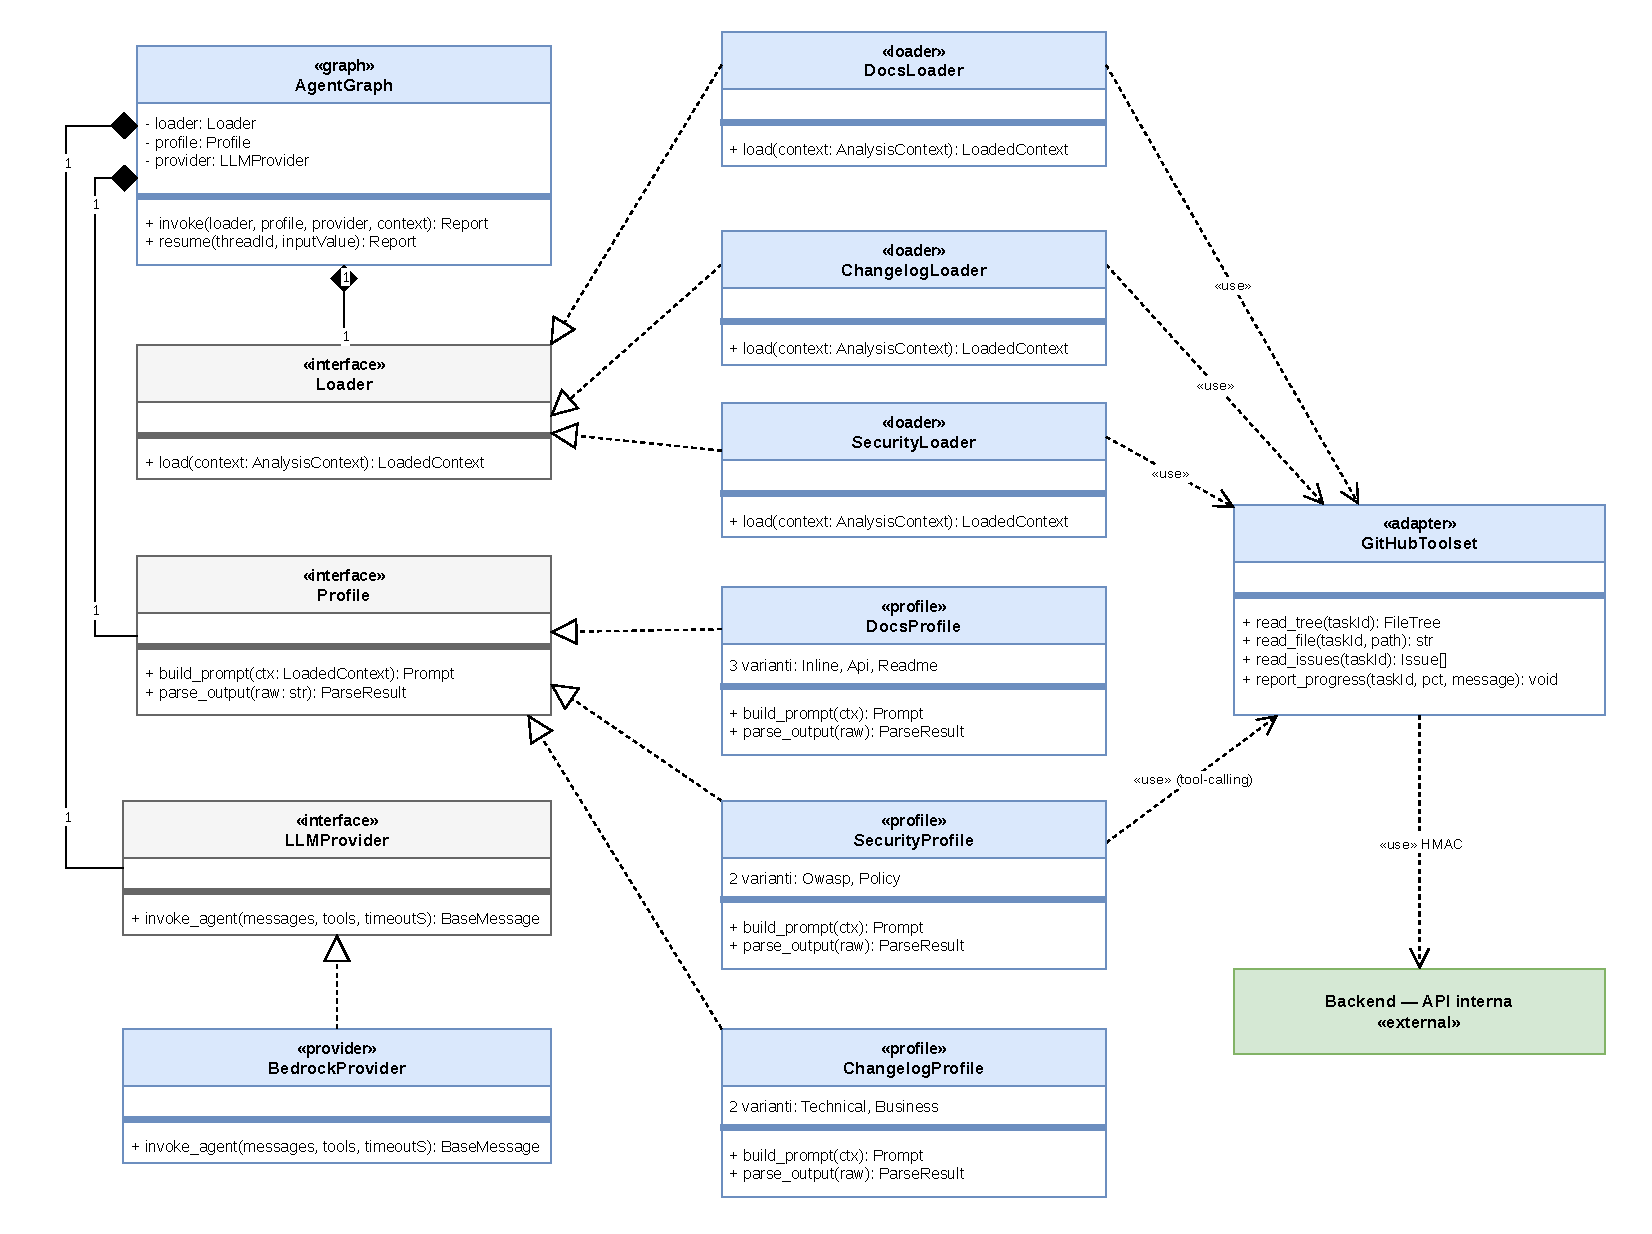
\includegraphics[width=0.95\textwidth]{agenti-architettura.pdf}
    \caption{AgentGraph: un solo scheletro, tre configurazioni}
    \label{fig:agenti-architettura}
\end{figure}

Tutte e tre le configurazioni condividono anche lo stesso adattatore verso l'esterno, \texttt{GitHubToolset}: è la controparte, lato agente, della facade di sola lettura già descritta nell'integrazione con GitHub. Ogni chiamata è firmata con lo stesso schema HMAC verificato da \texttt{InternalAuthGuard}, e non porta con sé proprietario e nome del repository: viaggia solo l'identificativo della Task, dal quale il Backend risolve il contesto reale. Un agente non può quindi accedere a un repository diverso da quello della propria Task.

La granularità reale è più fine di quanto suggerisca parlare di "tre agenti": ogni operazione ha il proprio \texttt{Profile}, per un totale di sette classi anziché tre. Farne convivere più d'una in un unico profilo parametrizzato avrebbe significato condizionare la costruzione del prompt e l'interpretazione della risposta sul tipo di operazione, con classi meno mirate e più difficili da testare in isolamento. Con un profilo per operazione, invece, aggiungerne una nuova significa aggiungere una classe, non modificarne una esistente. I template dei prompt seguono lo stesso principio di separazione: vivono come file esterni al codice invece che incorporati nelle classi Profile, e la logica che li carica e che estrae il JSON dalla risposta del modello è la stessa per tutti. Ogni Profile si limita a indicare quale file usare per la propria operazione.

\subsubsection{Il grafo di esecuzione}

Ogni invocazione attraversa una sequenza fissa di fasi: caricamento del contesto tramite il Loader, composizione del prompt tramite il Profile, invocazione del modello e, quando il Profile lo prevede, uno o più cicli di chiamata a strumenti esterni prima di ottenere una risposta definitiva. L'unico agente che usa strumenti durante l'esecuzione, anziché solo in fase di caricamento del contesto, è l'Agente Security: il modello può richiedere di leggere altri file del repository mentre valuta una vulnerabilità o una violazione di policy, entro un numero massimo di cicli oltre il quale l'esecuzione viene comunque chiusa come fallita.

L'output del modello non viene persistito così com'è: passa prima per una fase di validazione che, in caso di errore, non fallisce subito ma corregge. Un output che non è JSON valido viene ripresentato al modello insieme a un prompt correttivo, fino a un numero massimo di tentativi. L'Agente Changelog, nella sua variante rivolta al business, applica lo stesso principio a un problema diverso: se il testo prodotto risulta troppo complesso secondo l'indice di leggibilità Flesch, chiede al modello di riscriverlo in modo più semplice, spiegandogli concretamente cosa rende un testo più leggibile. L'esecuzione termina in un fallimento vero e proprio solo quando anche i tentativi di correzione si esauriscono.

\subsubsection{Sospensione e ripresa}

Anche mentre attende un input, una Task resta nello stato \texttt{RUNNING}. La sospensione non aggiunge uno stato: è una condizione interna, segnalata dal campo \texttt{pendingInput}. Il campo descrive cosa manca, non lo contiene ancora: il Frontend ne legge il tipo per scegliere quale finestra proporre, mentre la risposta effettiva dell'utente (un valore vero e proprio nel caso dello Sprint ID, una conferma o un rifiuto negli altri due casi) viaggia separatamente su \texttt{POST /tasks/:id/input}, che azzera \texttt{pendingInput} e rimette in coda la Task.

\begin{figure}[H]
    \centering
    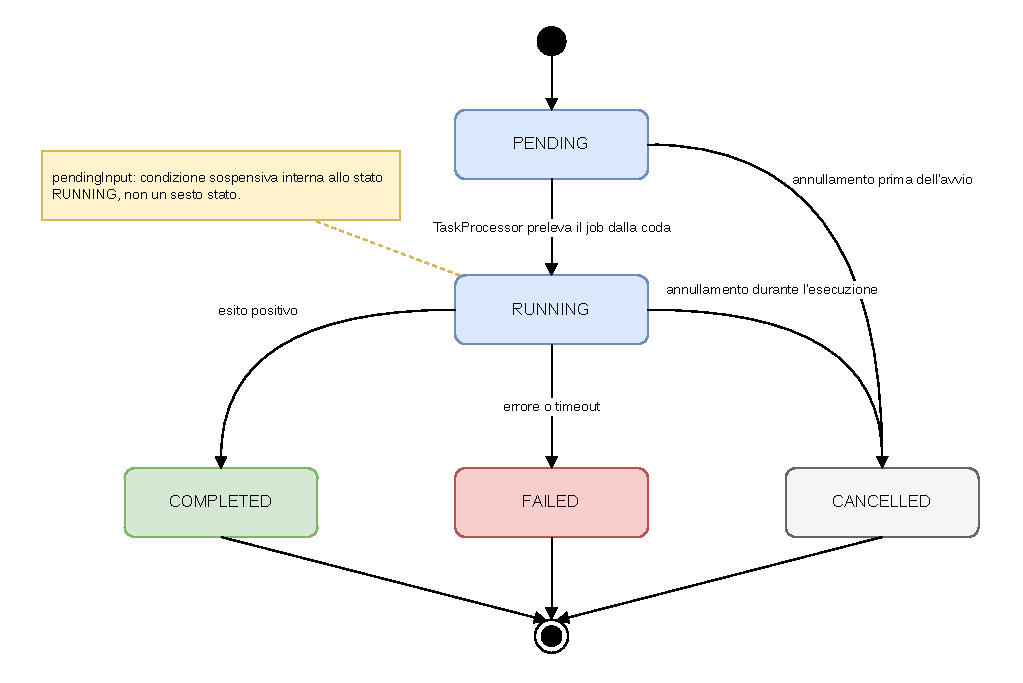
\includegraphics[width=0.8\textwidth]{agenti-task-lifecycle.pdf}
    \caption{Ciclo di vita della Task.}
    \label{fig:agenti-lifecycle}
\end{figure}

L'Agente Changelog è l'unico che può richiedere questo tipo di sospensione, fino a tre volte nel corso di una singola Task. La prima non ha nulla a che fare con il grafo dell'agente, che a quel punto non è ancora stato invocato: entrambe le operazioni Changelog richiedono uno Sprint ID, ed è il Backend stesso a sospendere la Task e a chiederlo, prima ancora di avviare l'agente. Le altre due sospensioni avvengono dentro un grafo già in esecuzione. Nella prima, se lo \texttt{ChangelogLoader} trova Issue chiuse con metadati insufficienti, l'agente si sospende subito e lascia all'utente la scelta se procedere escludendole o annullare la Task. Nella seconda, prevista solo per il changelog di business, l'agente si sospende appena completata internamente la fase tecnica, prima di passare alla fase business: l'intenzione è che l'utente possa rivedere il changelog tecnico prima di confermare. \emph{[Punto aperto: la fase tecnica non viene persistita come Report a sé stante prima di questa sospensione, poiché fa ancora parte dello stesso grafo non concluso; il riferimento pensato per permettere quella lettura non viene quindi valorizzato, e oggi la conferma avviene senza una reale anteprima.]}

Le sospensioni interne al grafo si appoggiano a un meccanismo di checkpoint di LangGraph, che salva lo stato interno del grafo su MongoDB a ogni passaggio: la stessa istanza usata per i dati applicativi, ma in collezioni gestite interamente da LangGraph e indipendenti dal modello di dominio della Figura \ref{fig:modello-dati}. È la scrittura su MongoDB già anticipata nella vista d'insieme, e permette di riprendere un'esecuzione esattamente dal punto in cui si era fermata. In tutti e tre i casi il Backend, ricevuta la risposta dell'utente, rimette la Task sulla stessa coda usata per un avvio normale; cambia solo l'endpoint con cui invoca il servizio agenti: \texttt{/internal/agent/start} se il grafo deve partire per la prima volta (Sprint ID), \texttt{/internal/agent/resume} con lo stesso \texttt{threadId} di prima se deve riprendere da un checkpoint (le altre due).

\subsubsection{Analisi statica con Semgrep}

Affidare la scansione di sicurezza al solo giudizio del modello linguistico espone a due rischi concreti: un tasso di falsi positivi più alto e un risultato non del tutto riproducibile, per via dell'indeterminismo degli LLM. Per questo, solo nella scansione OWASP, il Servizio Agenti affianca al giudizio del modello Semgrep, un motore di analisi statica deterministico eseguito come processo separato entro un tempo massimo. Le regole applicate combinano un insieme fisso orientato alla OWASP Top 10 con le regole specifiche per i linguaggi effettivamente presenti nel repository. Se Semgrep supera il proprio limite di tempo, l'agente non fallisce l'intera scansione ma prosegue con la sola analisi del modello, segnalandolo nel report.

Ogni segnalazione di Semgrep passa comunque al giudizio del modello, che restituisce per ciascuna un verdetto (confermata, falso positivo, o da rivedere) insieme a un rimedio per quelle confermate. Una segnalazione che il modello non commenta esplicitamente non viene accettata in silenzio: resta segnata come da rivedere. Il modello è inoltre libero di segnalare per conto proprio vulnerabilità che un'analisi statica non può cogliere, come un difetto di logica applicativa, indipendentemente da cosa abbia trovato Semgrep.

\subsection{Modello dei Dati Persistiti}
\label{subsec:modello-dati}

I dati applicativi persistono su MongoDB in sette collezioni, organizzate attorno a un'unica entità centrale: la Task. Ogni altra collezione o riferisce una Task, o è ciò da cui una Task viene generata.

\begin{figure}[H]
    \centering
    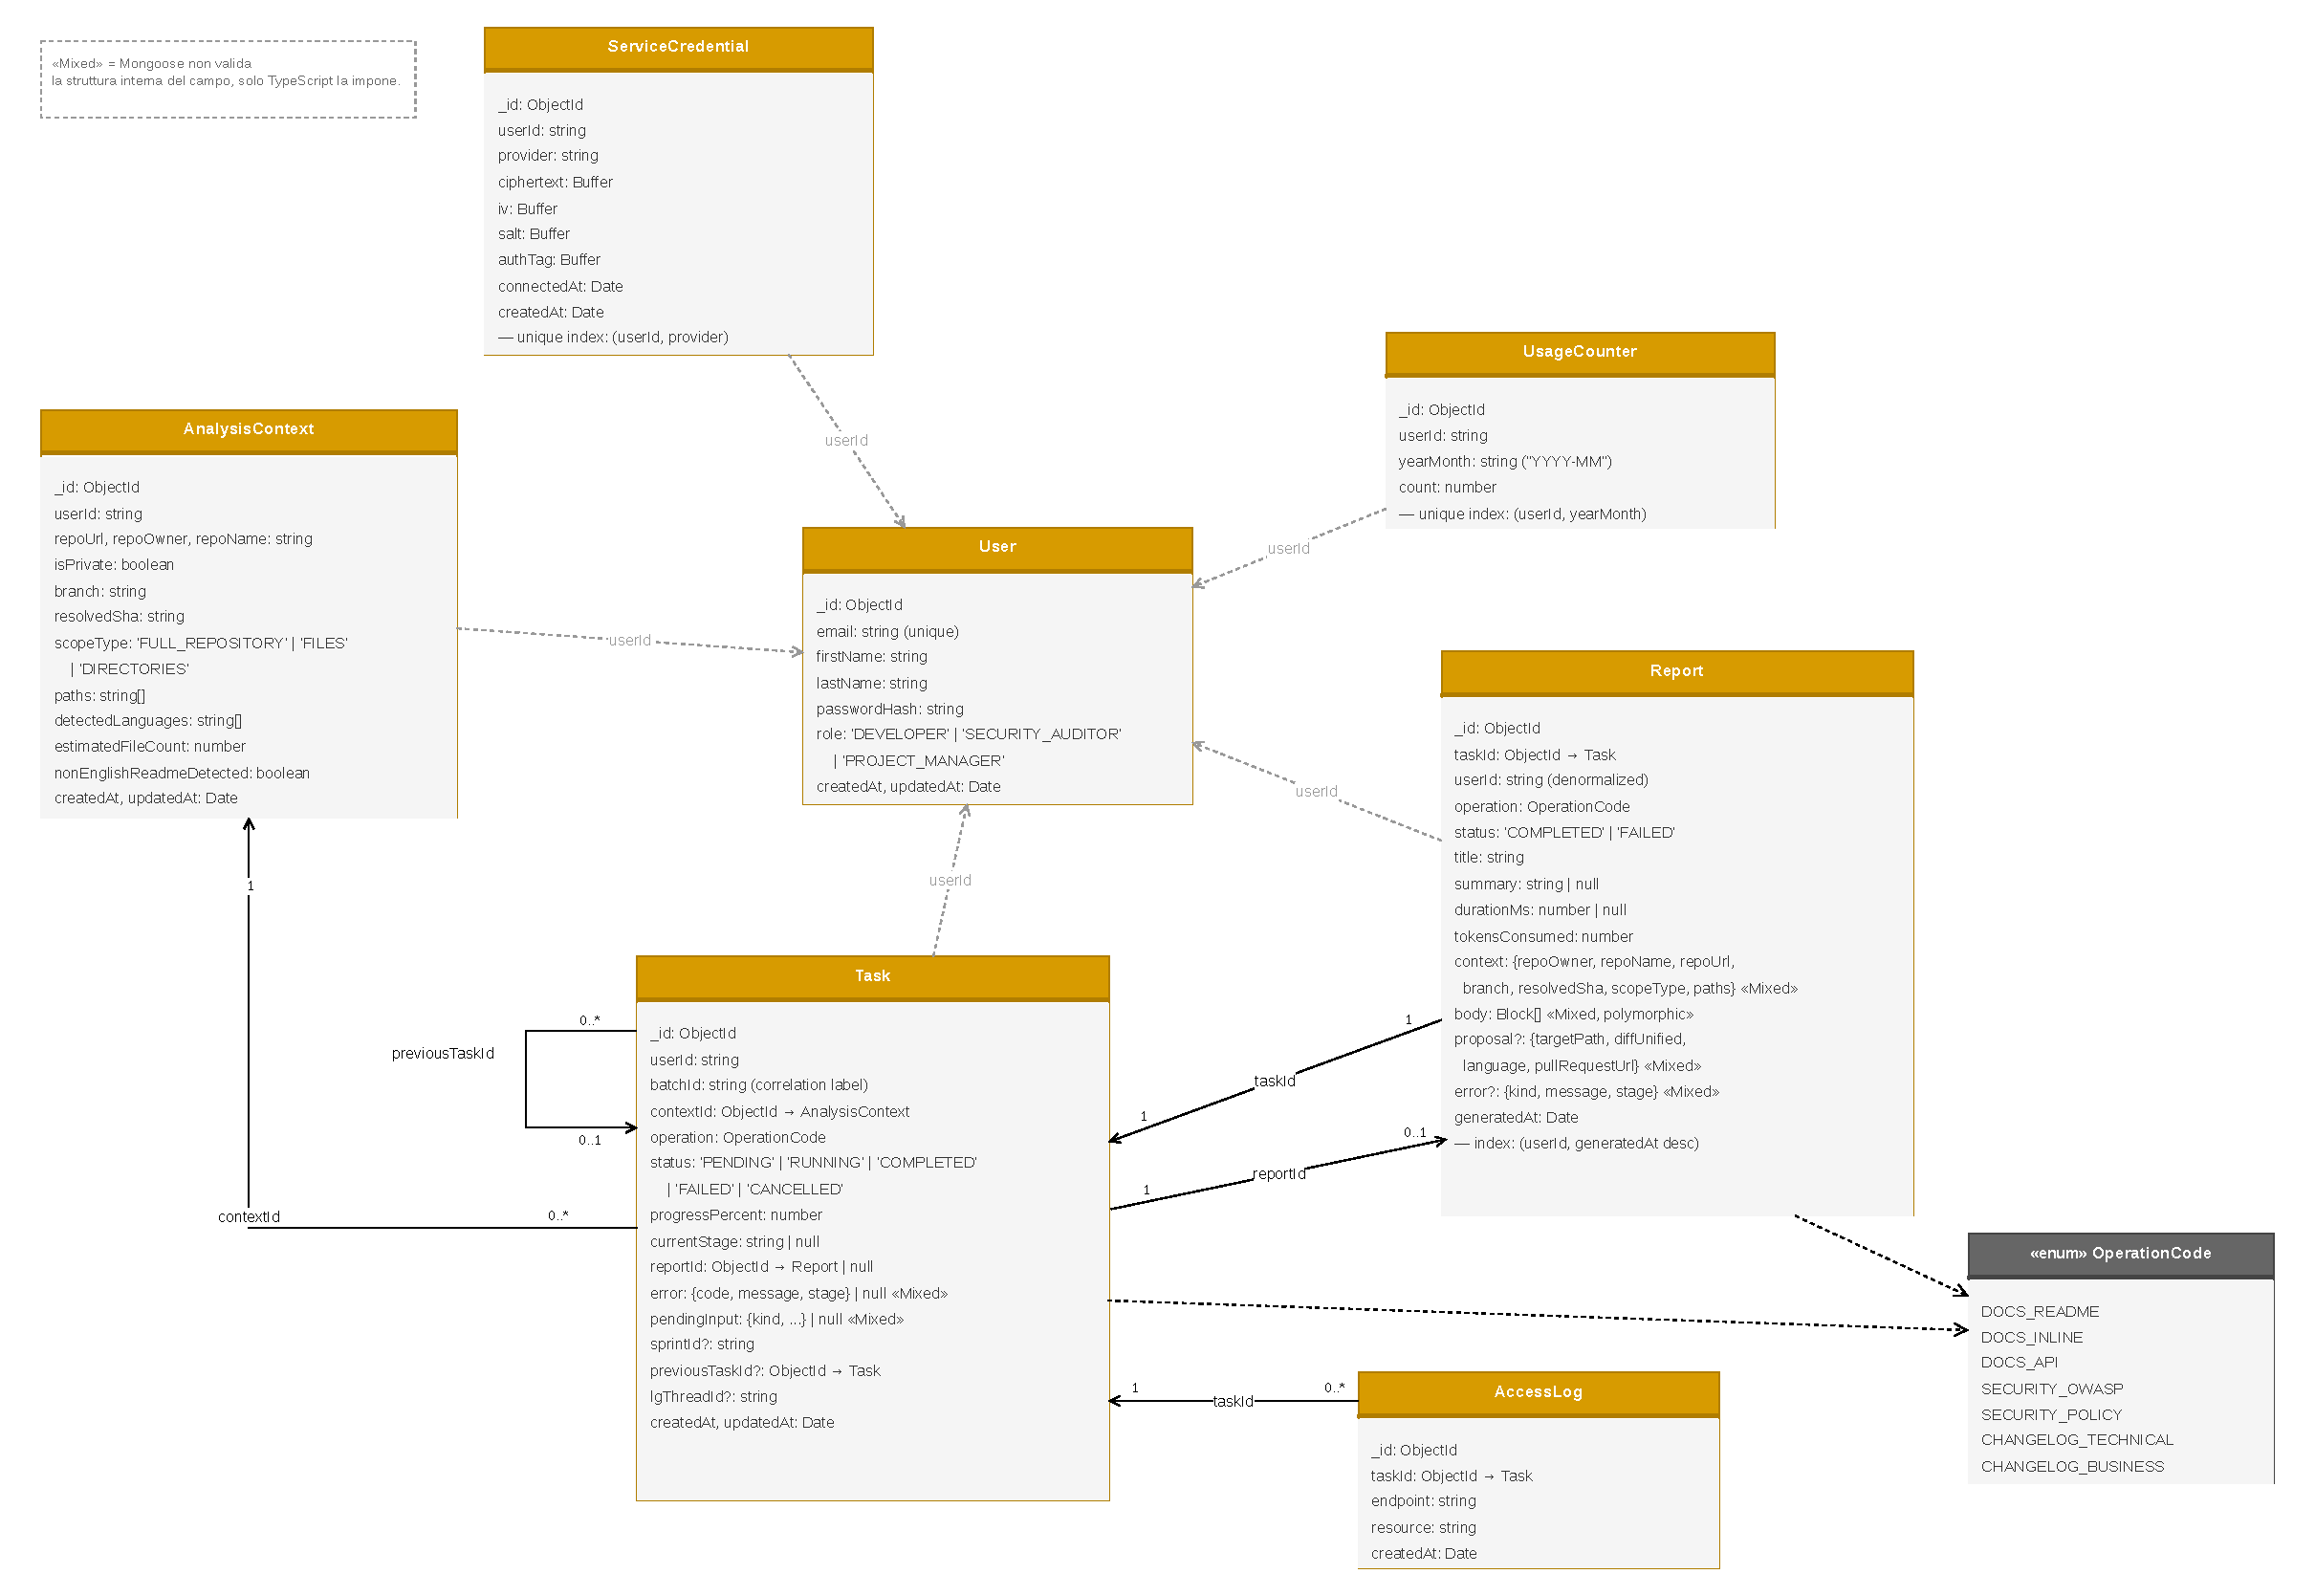
\includegraphics[width=0.95\textwidth]{modello-dati.pdf}
    \caption{Modello dei dati persistiti su MongoDB.}
    \label{fig:modello-dati}
\end{figure}

Le associazioni con l'utente proprietario, presenti su quasi ogni collezione, non sono riferimenti ma un semplice campo \texttt{userId} duplicato. Abbiamo scelto così perché ogni controllo di appartenenza diventa una lettura indicizzata su una singola collezione, invece di una \emph{join} tra due: operazione che MongoDB non offre nativamente allo stesso costo di un database relazionale.

Alcuni campi, in particolare \texttt{Task.error}, \texttt{Task.pendingInput} e gran parte di \texttt{Report} (\texttt{context}, \texttt{body}, \texttt{proposal}, \texttt{error}), sono persistiti come tipo \texttt{Mixed}: Mongoose li salva così come arrivano, senza validarne la struttura interna a livello di schema. Non è però solo il tipo TypeScript a garantire che quei valori abbiano la forma attesa, il corpo del Report è prima validato contro i modelli Pydantic del Servizio Agenti, che lo producono, e poi sanificato lato Backend. Il testo Markdown proveniente dal modello linguistico viene ripulito da destinazioni pericolose (ad esempio URL \texttt{javascript:}) prima di essere persistito, così che un output malevolo o malformato del modello non attraversi indisturbato il confine tra i due servizi.

Due indici composti univoci vincolano a livello di database due invarianti che, altrimenti, resterebbero affidati alla sola disciplina applicativa: \texttt{ServiceCredential} ammette una sola credenziale per coppia utente/provider, e \texttt{UsageCounter} un solo contatore per coppia utente/mese solare. Un terzo indice, non univoco, su \texttt{Report(userId, generatedAt)} riduce lo storico dei report a una singola lettura ordinata, invece di una scansione completa della collezione.

\newpage
\section{Design Pattern Implementati}

Il sistema si appoggia su un piccolo numero di design pattern, scelti perché ciascuno risolve un problema concreto incontrato durante la progettazione. Le sottosezioni seguenti li presentano uno per uno: il problema che chiudono, dove vivono nel codice, e perché li abbiamo preferiti alle alternative più semplici.

\subsection{Strategy}

\texttt{AgentGraph} deve eseguire tre agenti strutturalmente diversi senza duplicare, per ciascuno, la stessa logica di orchestrazione. Condizionare quella logica sul tipo di agente, con un ramo per Docs, uno per Security e uno per Changelog, l'avrebbe accoppiata a ogni agente esistente e a ogni agente futuro.

Il problema è chiuso da tre interfacce, \texttt{Loader}, \texttt{Profile} e \texttt{LLMProvider}, di cui \texttt{AgentGraph} riceve un'istanza dal proprio costruttore e a cui delega senza costruirle né conoscerne il tipo concreto. La scelta di quale coppia \texttt{Loader}/\texttt{Profile} usare, e di quale \texttt{LLMProvider}, avviene interamente fuori dal grafo, in base al codice operazione (Figura \ref{fig:agenti-architettura}).

Cambiare la configurazione di un agente non richiede quindi nessuna modifica ad \texttt{AgentGraph}: passare da un provider all'altro è un cambio di configurazione, non di codice, e ogni \texttt{Profile} si può testare in isolamento iniettando un provider simulato al posto di quello reale.

\subsection{Dependency Injection}

Un componente che costruisce da sé le proprie dipendenze è difficile da testare in isolamento e da adattare a un ambiente diverso da quello per cui è stato scritto. Un client Bedrock reale non si può sostituire con uno simulato se è il componente stesso a istanziarlo.

Sul Backend la dependency injection è quella nativa di NestJS, automatica tramite costruttore. Sul Servizio Agenti, che non ha un framework equivalente, applichiamo la stessa disciplina a mano: l'endpoint \texttt{/internal/agent/start} compone l'intero grafo di dipendenze prima di avviare l'esecuzione. Costruisce \texttt{SASTAnalyzer} e lo passa a \texttt{SecurityLoader}, poi passa \texttt{Loader}, \texttt{Profile} e \texttt{LLMProvider} già pronti al costruttore di \texttt{AgentGraph}, senza che nessuno di questi componenti costruisca da sé ciò di cui ha bisogno.

Il vantaggio è lo stesso su entrambi i lati: ogni componente si testa iniettando un mock al posto della dipendenza reale, e l'intero grafo delle dipendenze resta visibile e modificabile in un unico punto invece che sparso nei costruttori di ciascuna classe.

\subsection{Facade}

L'API REST di GitHub espone una superficie ampia e facile da usare male direttamente: paginazione da gestire a mano, forme di risposta verbose, endpoint diversi per l'albero dei file, un singolo file, un branch, un confronto tra commit, le issue. Backend e Servizio Agenti hanno bisogno solo di un piccolo sottoinsieme coerente di tutto questo.

\texttt{GithubClientService} unifica le operazioni di lettura dietro metodi mirati e già semplificati nella forma del dato restituito; \texttt{GithubWriteService} fa lo stesso per la scrittura, riusando \texttt{GithubClientService} solo per le proprie letture di supporto (Figura \ref{fig:backend-github}).

Nessun altro punto del sistema ha bisogno di conoscere la forma delle risposte di GitHub. La separazione tra le due classi ha poi una seconda conseguenza, strutturale: un agente non può aggirare il vincolo di sola lettura. Il confine passa per \texttt{InternalGithubController}, l'unico punto che gli agenti raggiungono, e il suo costruttore riceve in iniezione soltanto \texttt{GithubClientService}, mai \texttt{GithubWriteService}.


\subsection{Adapter}

Durante l'esecuzione l'agente deve poter leggere contenuti dal repository, ma non può parlare direttamente con GitHub: può raggiungere solo l'API interna del Backend, autenticata via firma HMAC.

\texttt{GitHubToolset} adatta l'intera interazione con quell'API (costruzione della richiesta, firma HMAC, chiamata di rete, interpretazione della risposta) dietro un piccolo insieme di metodi locali, invocabili come funzioni ordinarie e non come chiamate HTTP: \texttt{read\_tree}, \texttt{read\_file}, \texttt{read\_issues}, \texttt{report\_progress}. Tutti i dettagli del protocollo restano nascosti dentro un unico metodo privato (Figura \ref{fig:agenti-architettura}).

Il resto del codice dell'agente chiama questi metodi senza sapere che dietro c'è una chiamata di rete firmata: cambiare lo schema di firma o la forma degli endpoint interni resterebbe confinato a questa sola classe.

\newpage
\section{Flusso dei dati}

Le sezioni precedenti descrivono la struttura del sistema: quali componenti esistono, come sono organizzati, quali collegamenti sono ammessi tra loro. Qui la stessa architettura si vede in movimento. Seguiamo passo per passo sei scenari concreti, ciascuno scelto perché mette in gioco un meccanismo diverso tra quelli già introdotti, nell'ordine in cui un utente li incontrerebbe davvero: la connessione della credenziale GitHub, senza la quale nessuna delle fasi successive è possibile; la creazione del contesto di analisi; l'avvio e il completamento di un'operazione nel caso generale; la lettura del repository durante l'esecuzione di un agente; la sospensione dell'Agente Changelog in attesa di una decisione umana; e infine l'esportazione di un Report in PDF.

\subsection{Connessione delle credenziali}
\label{subsec:flusso-credenziali}

Il primo scenario è il primo passo che l'utente deve completare: senza una credenziale GitHub configurata, nessuna delle fasi successive può nemmeno iniziare, perché è da questa credenziale che ogni chiamata a GitHub del Backend parte.

\begin{figure}[H]
    \centering
    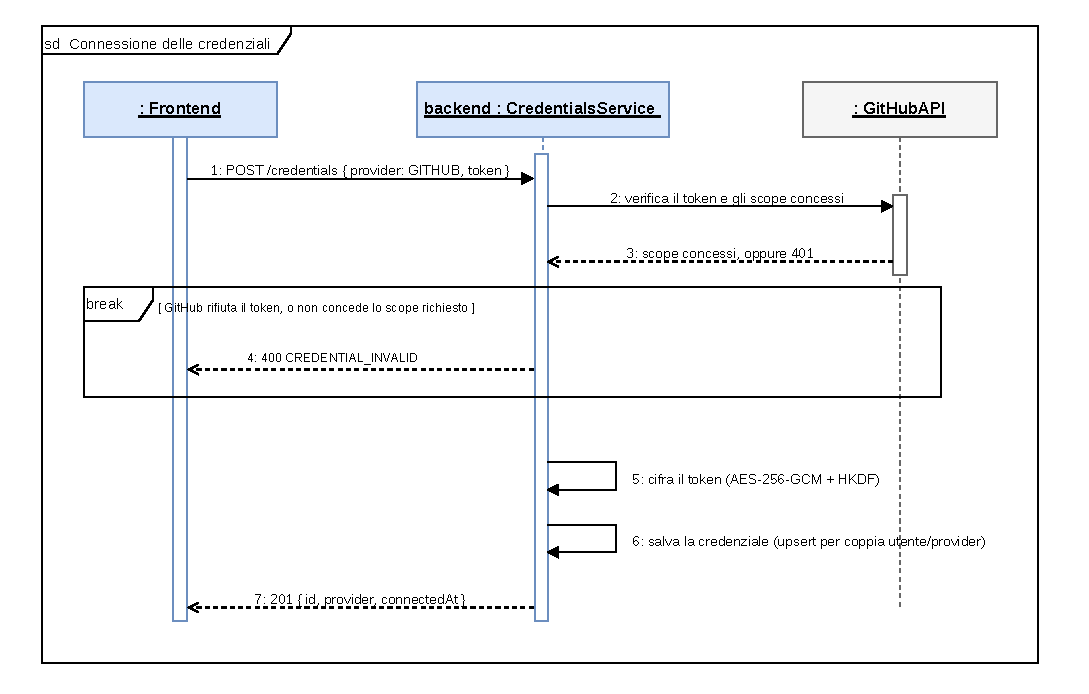
\includegraphics[width=0.95\textwidth]{flusso-credenziali.pdf}
    \caption{Connessione di una credenziale GitHub.}
    \label{fig:flusso-credenziali}
\end{figure}

Il token non viene cifrato e salvato sulla fiducia: prima ancora di toccare lo schema di cifratura già descritto in \S~\ref{subsec:backend}, il Backend lo usa per interrogare GitHub e verificare che sia valido e che conceda lo scope richiesto. Solo un token che supera questo controllo dal vivo arriva a essere cifrato e persistito; uno rifiutato da GitHub non produce alcuna scrittura. Conta anche cosa \emph{non} viene trattato come credenziale non valida: un errore di rete o un problema temporaneo lato GitHub restano un guasto a monte (\texttt{UPSTREAM}), non un giudizio sul token. Altrimenti un disservizio esterno indurrebbe l'utente a riconfigurare una credenziale che in realtà funziona.

\subsection{Creazione del contesto di analisi}
\label{subsec:flusso-contesto}

Il secondo scenario riguarda il passo immediatamente successivo: prima di poter scegliere e avviare un'operazione, l'utente deve fissare su cosa quell'operazione lavorerà, cioè creare un \texttt{AnalysisContext}.

\begin{figure}[H]
    \centering
    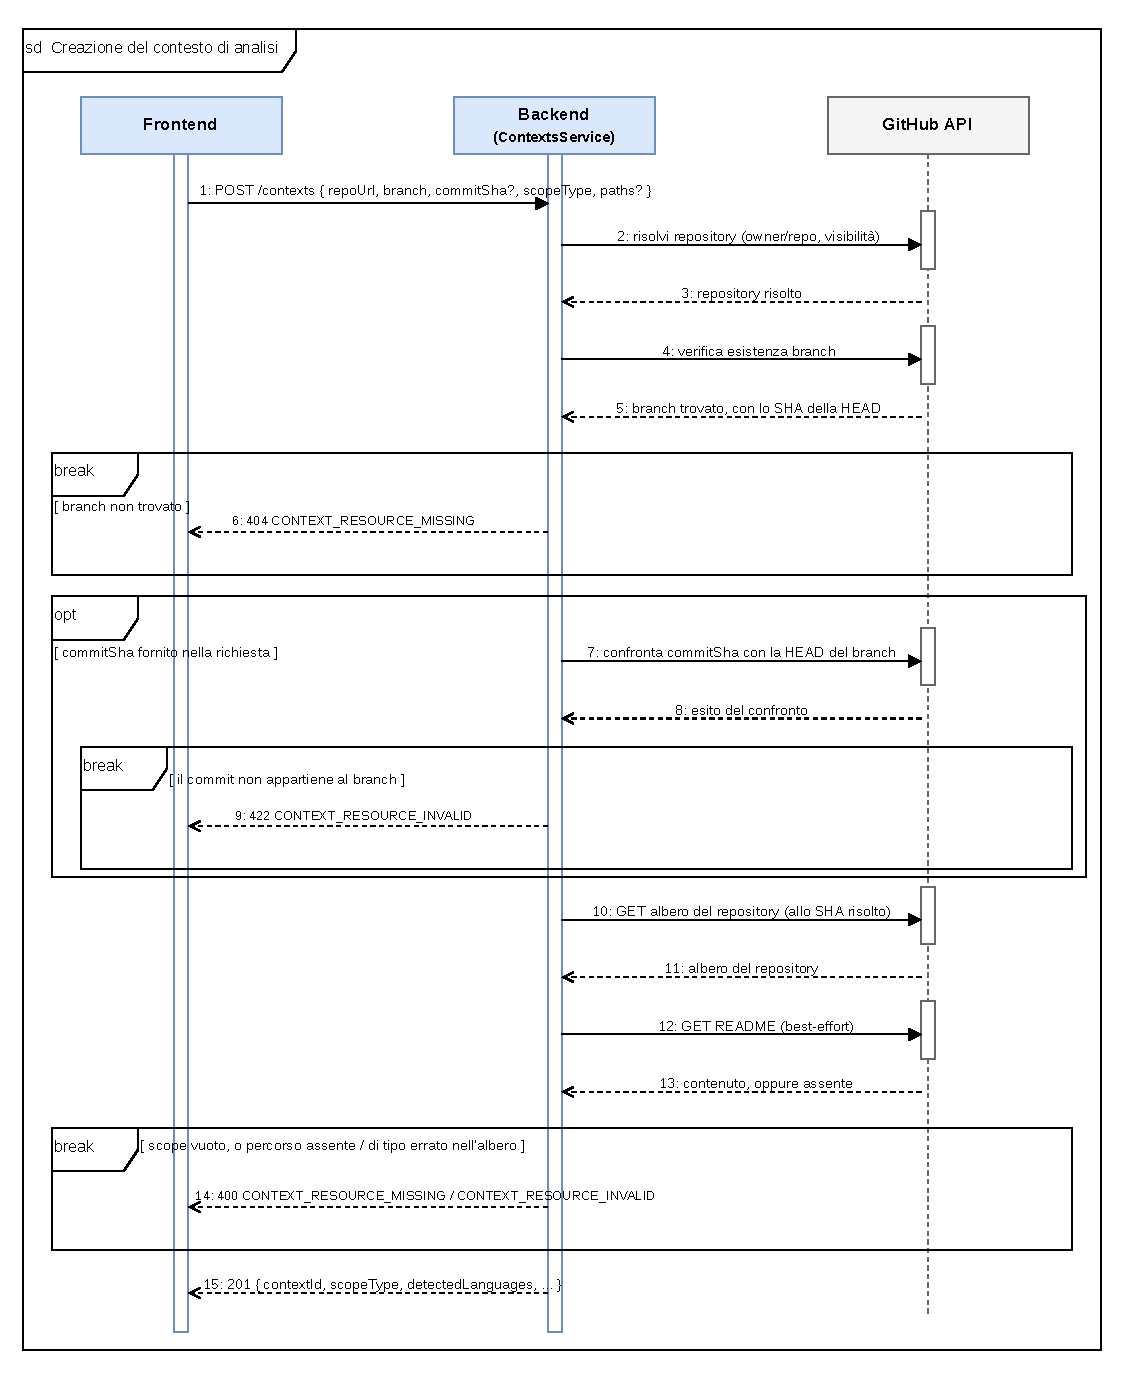
\includegraphics[width=1.0\textwidth]{flusso-creazione-contesto.pdf}
    \caption{Creazione del contesto di analisi.}
    \label{fig:flusso-contesto}
\end{figure}

La richiesta attraversa una sequenza fissa di controlli, ciascuno in grado di interromperla: l'esistenza del repository e del branch indicato, l'appartenenza dell'eventuale commit specificato a quel branch, e la validità dello scope scelto rispetto ai file realmente presenti nel repository. Nulla viene persistito finché non li supera tutti. Dall'elenco dei controlli sfuggono però due dettagli. Il riferimento non resta puntato su un branch in movimento: viene risolto una volta per tutte in uno SHA di commit preciso, in modo che lo stesso contesto continui a produrre lo stesso risultato anche dopo nuovi commit sul repository. E l'albero del repository viene letto una sola volta, perché quella stessa lettura serve sia a rilevare i linguaggi presenti sia a verificare che i percorsi dello scope esistano davvero: due controlli che partono dallo stesso dato non richiedono due interrogazioni a GitHub.

\subsection{Avvio ed esecuzione di un'operazione}
\label{subsec:flusso-avvio}

Il terzo scenario segue un'operazione che non richiede né chiamate a strumenti durante l'esecuzione né sospensioni, ad esempio la generazione del README di progetto: è la forma più semplice che ogni operazione condivide, e serve da riferimento prima di introdurre le due varianti più articolate nelle sezioni successive.

\begin{figure}[H]
    \centering
    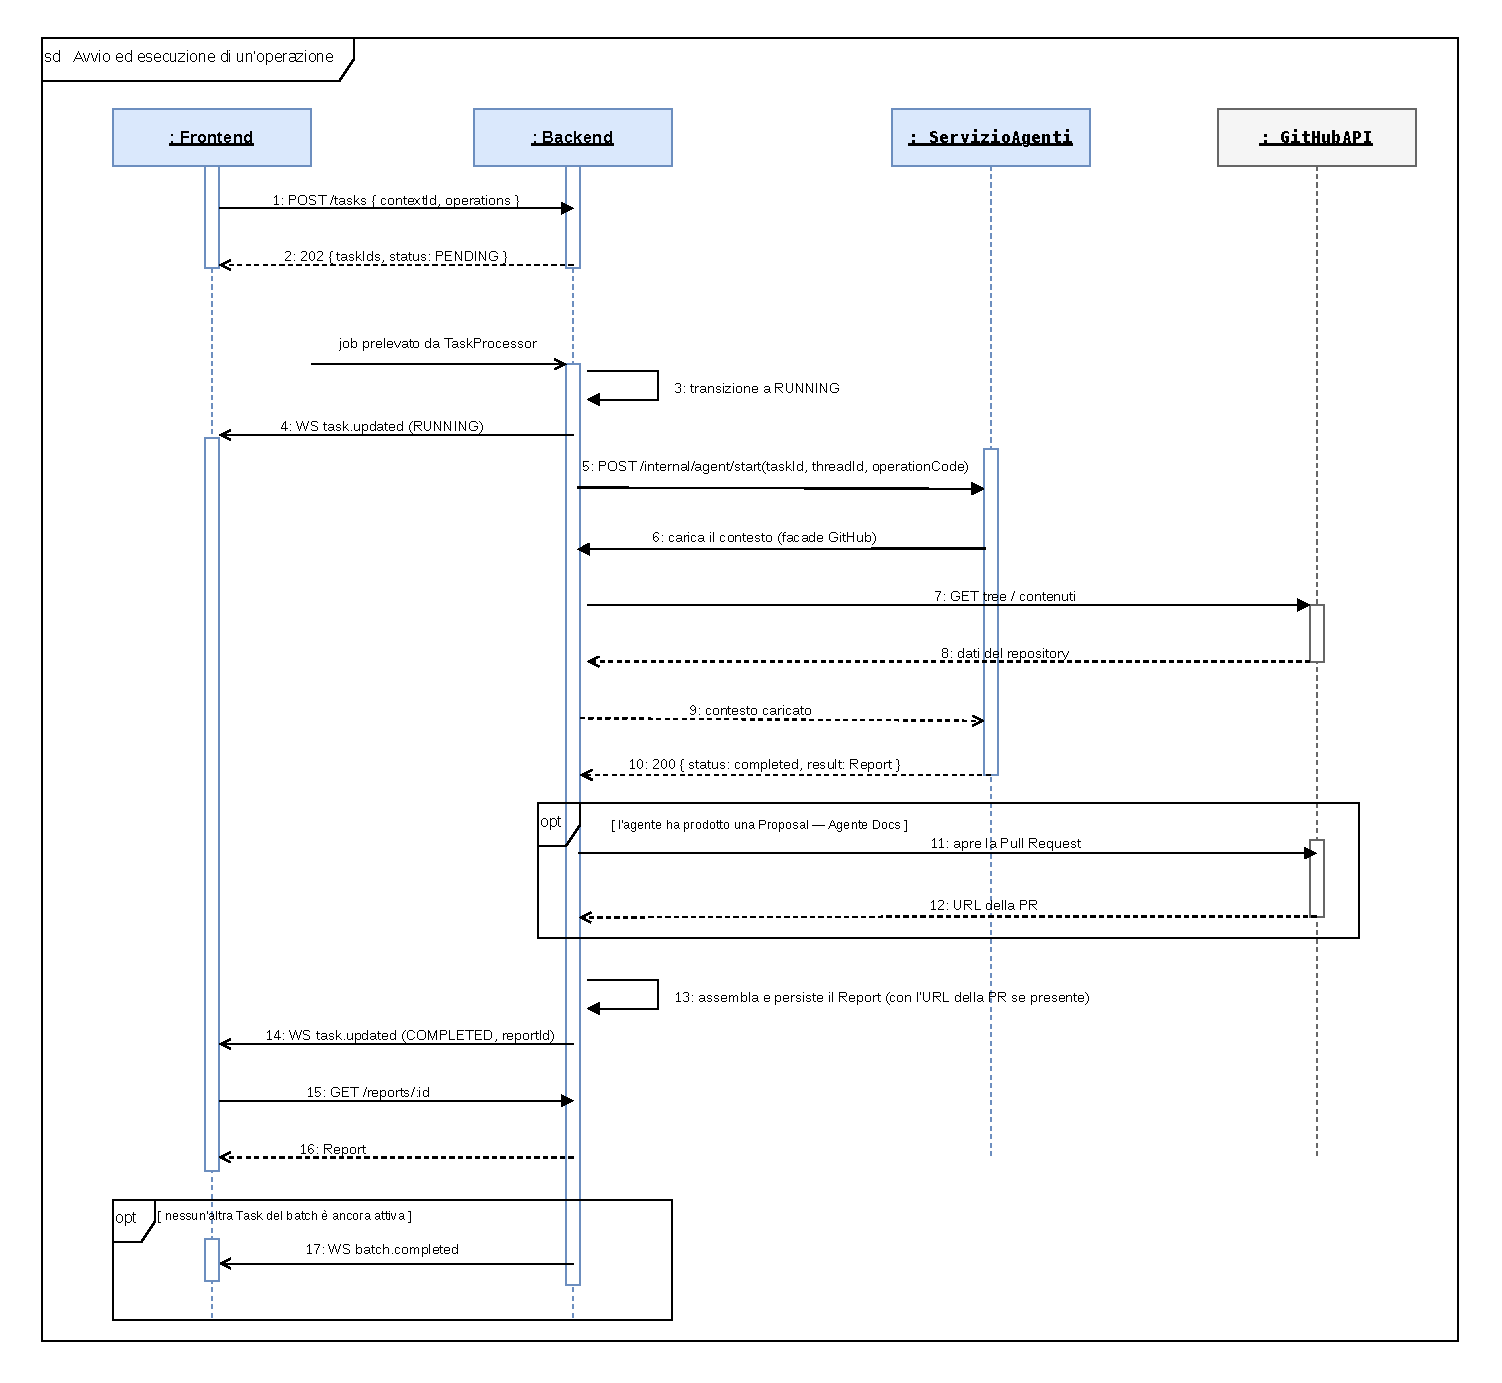
\includegraphics[width=1.0\textwidth]{flusso-avvio-generale.pdf}
    \caption{Avvio ed esecuzione di un'operazione nel caso generale.}
    \label{fig:flusso-avvio}
\end{figure}

La richiesta HTTP e l'esecuzione effettiva sono due momenti separati nel tempo. \texttt{POST /tasks} restituisce le Task appena create in stato \texttt{PENDING} senza attendere che nulla venga eseguito; solo più tardi, in un momento indipendente dal ciclo della richiesta, \texttt{TaskProcessor} preleva il job dalla coda e invoca il Servizio Agenti. Da quel punto in avanti tutta l'interazione con GitHub passa dal Backend, attraverso la stessa facade di sola lettura descritta in \S~\ref{subsec:backend}. Solo l'Agente Docs, tra i tre, fa seguire al completamento l'apertura automatica di una Pull Request; per gli altri due, il diagramma si fermerebbe un passo prima. L'ultimo tratto, dalla notifica \texttt{task.updated} alla lettura del Report, è lo stesso qualunque sia l'agente coinvolto, perché entrambi i lati trattano il risultato attraverso l'unico contratto \texttt{Report} già descritto in \S~\ref{subsec:backend}.

Il diagramma precedente tratta il Backend come un unico partecipante; la Figura~\ref{fig:flusso-avvio-dettaglio} rientra in quello stesso riquadro e mostra la sequenza reale tra le sue classi interne, già introdotte in \S~\ref{subsec:backend}.

\begin{figure}[H]
    \centering
    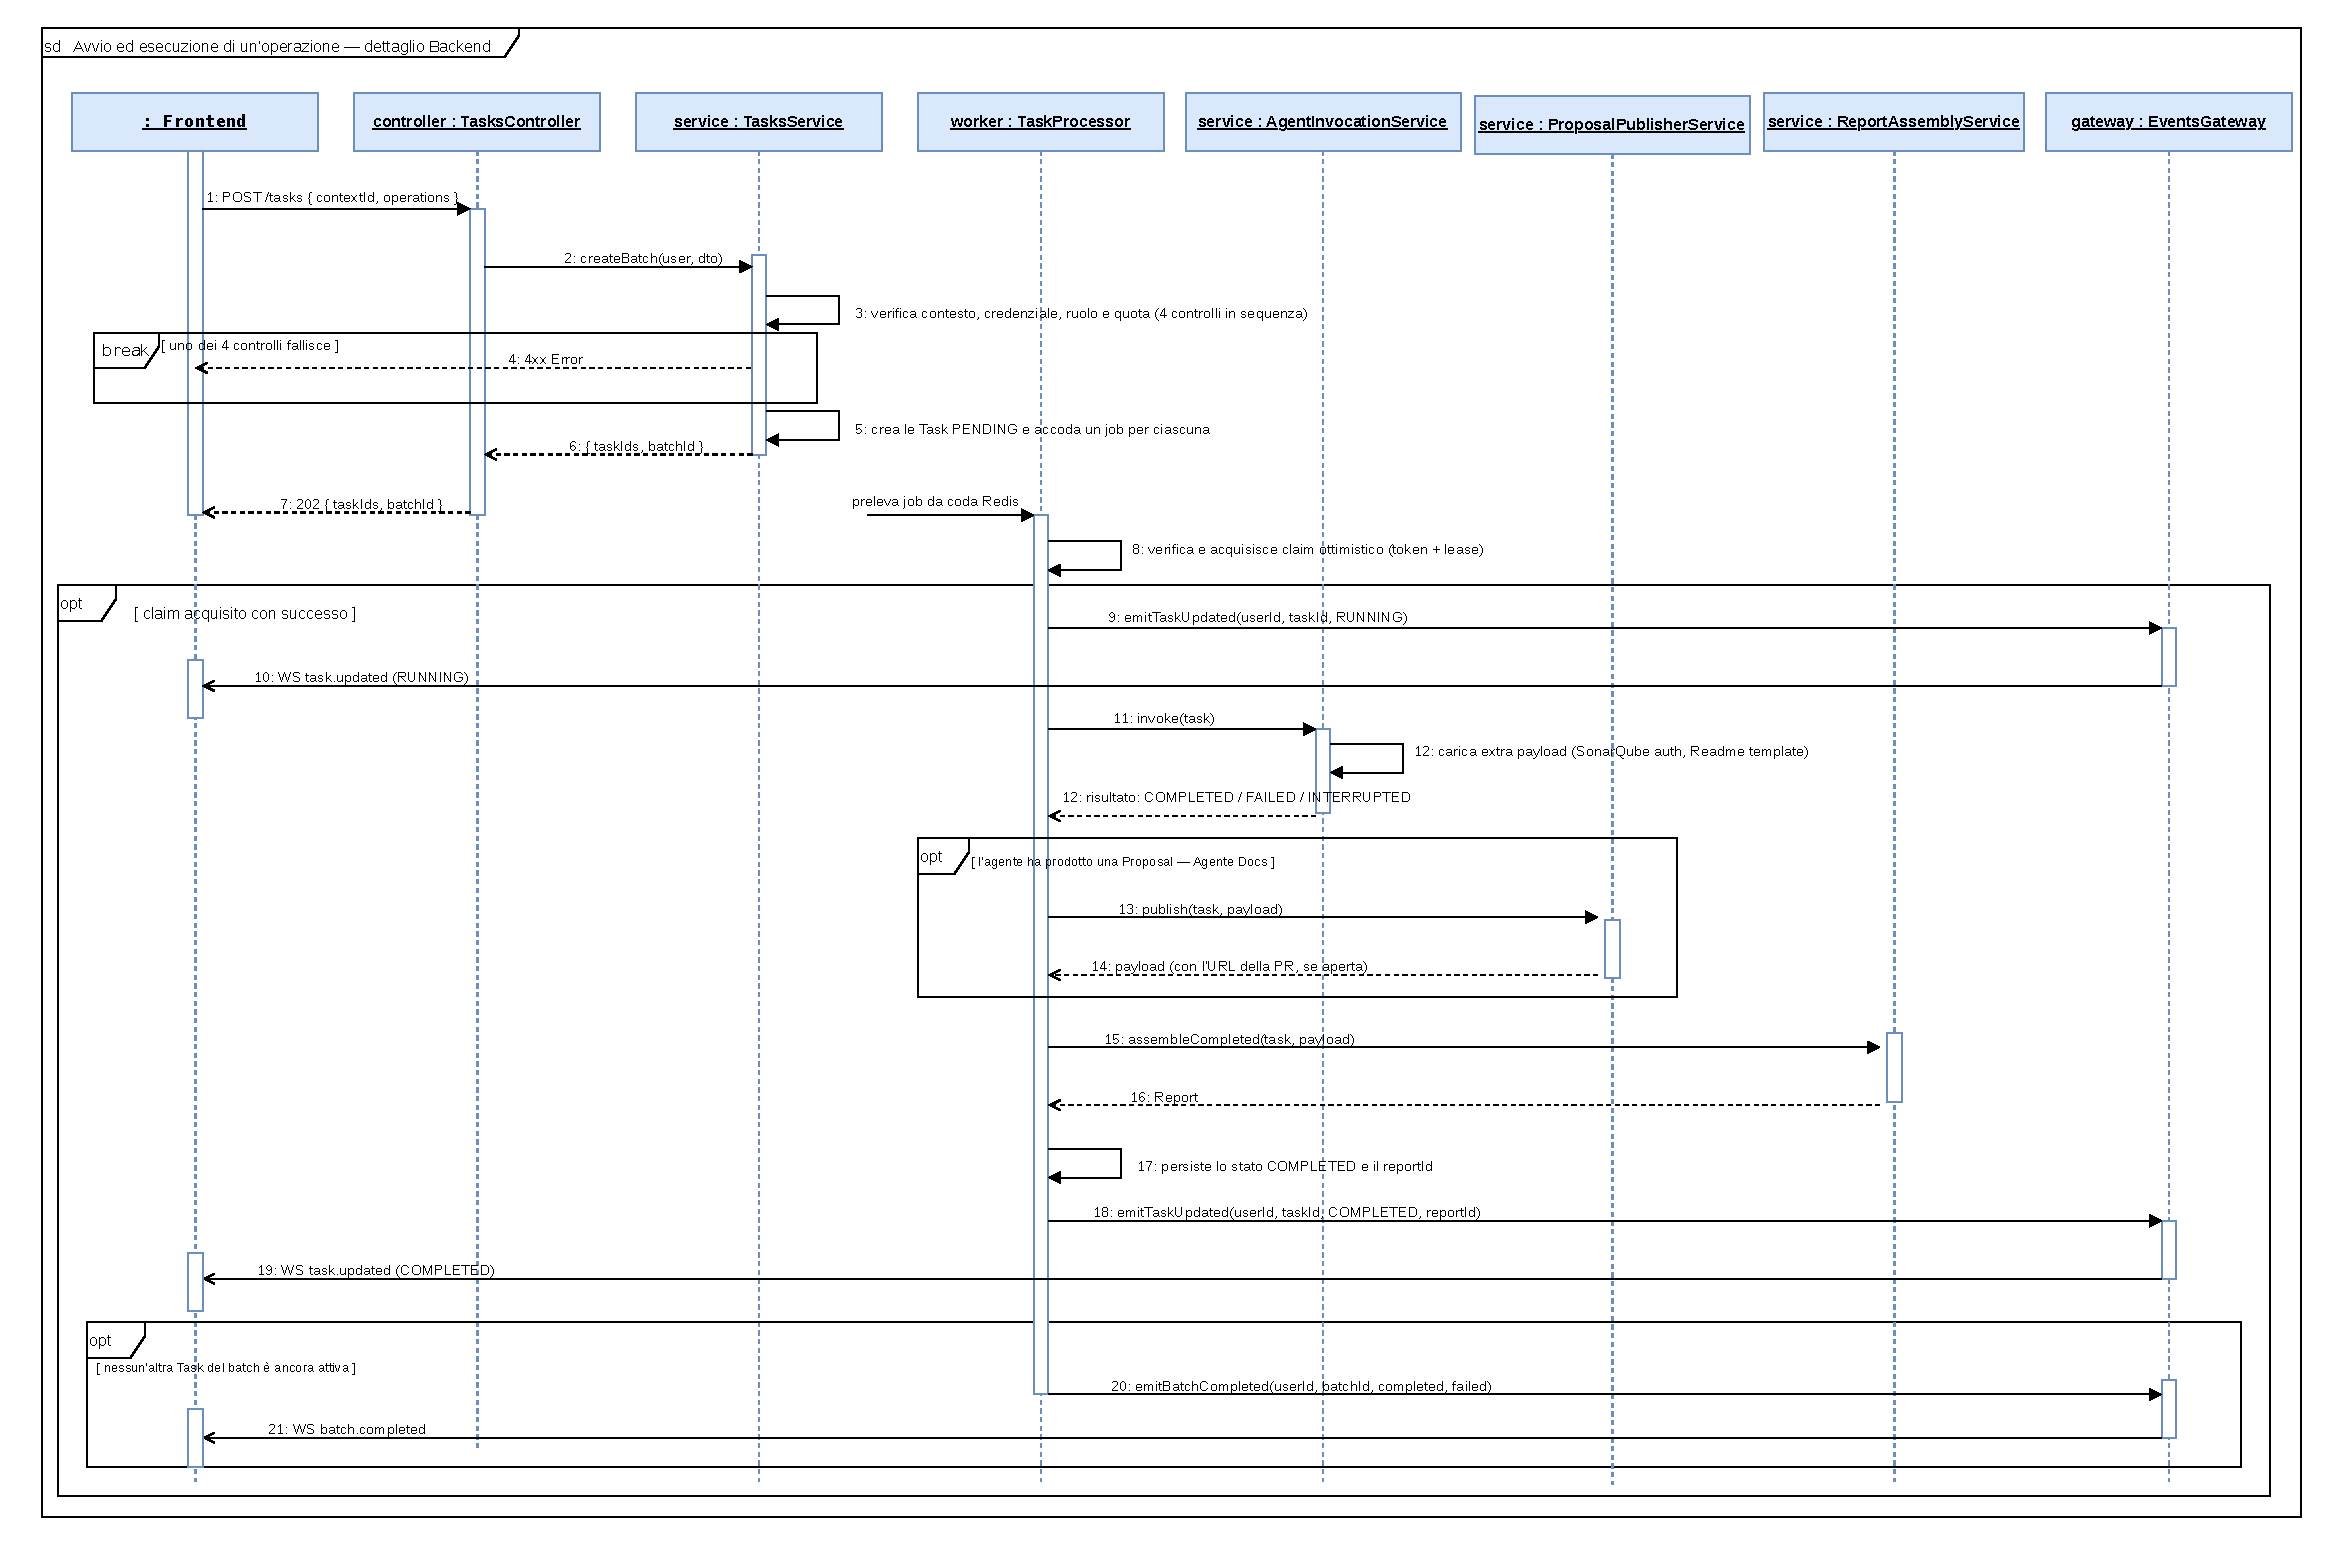
\includegraphics[width=1.0\textwidth]{flusso-avvio-dettaglio-backend.pdf}
    \caption{Avvio ed esecuzione di un'operazione: dettaglio delle classi interne del Backend.}
    \label{fig:flusso-avvio-dettaglio}
\end{figure}

Il confine tra i due momenti del flusso è visibile qui in una forma che il diagramma d'insieme non può mostrare. \texttt{TasksController} e \texttt{TasksService} non chiamano direttamente \texttt{TaskProcessor}, né lo attendono: scrivono in coda e restituiscono la risposta. È \texttt{TaskProcessor} a prelevare il job, in un momento scelto da lui e non da chi lo ha accodato. La prima cosa che fa, prima ancora di invocare l'agente, è segnalare al Frontend il passaggio a \texttt{RUNNING} tramite \texttt{EventsGateway}: quell'evento ha quindi una fonte distinta dal successivo \texttt{COMPLETED}.

Anche l'assemblaggio del Report, che il diagramma d'insieme tratta come un unico passo del Backend, si scompone qui in due classi con una responsabilità ciascuna e un ordine preciso tra loro: \texttt{ProposalPublisherService} apre la Pull Request quando l'agente ha prodotto una Proposal, e solo dopo \texttt{ReportAssemblyService} costruisce il Report, ricevendo un payload che già contiene l'URL della PR se questa è stata aperta. \texttt{AgentInvocationService} ed \texttt{EventsGateway} restano due classi distinte pur essendo entrambe invocate da \texttt{TaskProcessor}, perché rispondono a due domande diverse: la prima esegue l'operazione, la seconda ne comunica l'esito.

\subsection{Lettura del repository durante l'esecuzione: la scansione Security}
\label{subsec:flusso-tool-calling}

Il quarto scenario mostra cosa succede quando l'esecuzione non si limita a un solo giro di caricamento del contesto, ma continua a interrogare il repository mentre è già in corso: è il comportamento esclusivo dell'Agente Security, in entrambe le proprie operazioni. Le letture aggiuntive hanno qui due origini diverse, da non confondere. Una parte è decisa a priori dal Loader, prima ancora che il modello veda un prompt; un'altra è decisa dal modello stesso, durante il proprio ragionamento.

\begin{figure}[H]
    \centering
    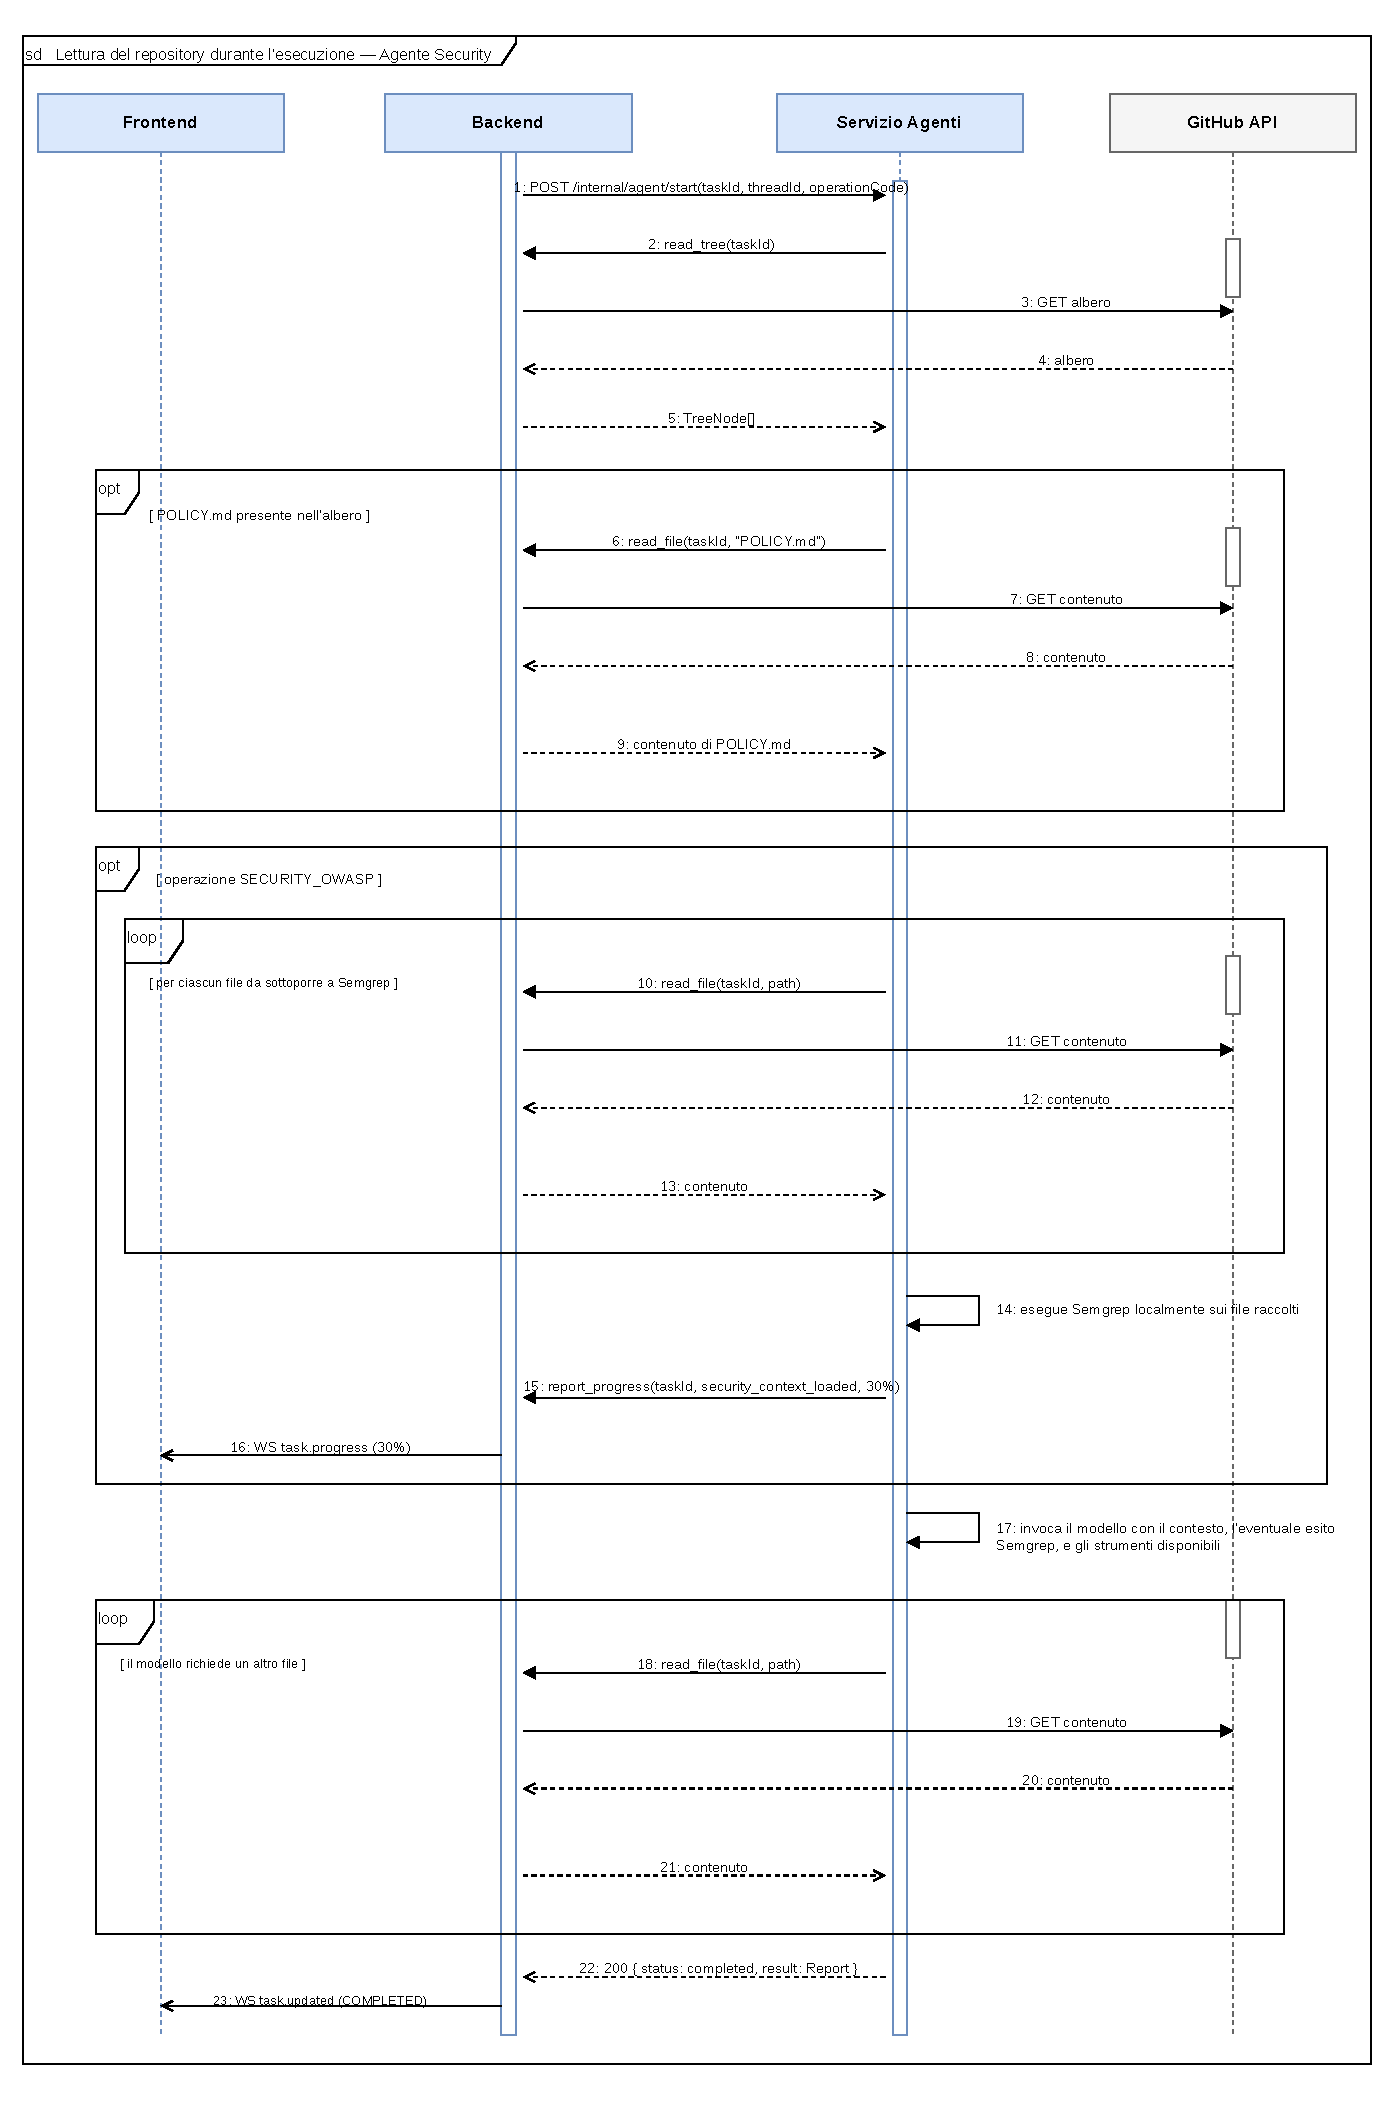
\includegraphics[width=1.0\textwidth]{agenti-sequenza-tool-calling.pdf}
    \caption{Le due fasi di lettura del repository durante l'esecuzione dell'Agente Security.}
    \label{fig:flusso-tool-calling}
\end{figure}

Dopo l'albero del repository, il \texttt{Loader} legge anche \texttt{POLICY.md} se presente, indipendentemente dall'operazione: nella scansione Policy il suo contenuto è la stessa direttiva da verificare, mentre nella scansione OWASP arricchisce semplicemente il prompt con eventuali regole aggiuntive del team. Solo per l'operazione OWASP segue poi una seconda lettura, questa volta non richiesta dal modello ma decisa interamente dal Loader: recupera il contenuto di ciascun file nello scope, fino a un numero massimo, per sottoporlo a Semgrep prima ancora di comporre il prompt. È a valle di questa fase, non prima, che il Servizio Agenti comunica il primo avanzamento della Task: il trenta per cento segnala che il contesto è pronto, esito di Semgrep compreso quando presente, non che l'esecuzione sia a un terzo del proprio percorso.

Solo da qui in avanti entra in gioco il modello, ed è solo lui a decidere se leggere altro: un file alla volta, per valutare una vulnerabilità o una violazione di policy, entro il numero massimo di cicli già descritto in \S~\ref{subsec:agenti}. Ogni lettura, in entrambe le fasi, attraversa comunque la stessa facade del Backend: cambiano il momento e chi la richiede, non il percorso.
\newpage
\subsection{Sospensione e ripresa: il changelog di business}
\label{subsec:flusso-sospensione}

Il quinto scenario segue l'unico caso in cui l'esecuzione si interrompe per attendere una decisione dell'utente durante lo svolgimento del grafo: la conferma richiesta prima di avviare la fase di business del changelog, già descritta in \S~\ref{subsec:agenti}. Il diagramma mostra le due uscite possibili da quella decisione fianco a fianco.

\begin{figure}[H]
    \centering
    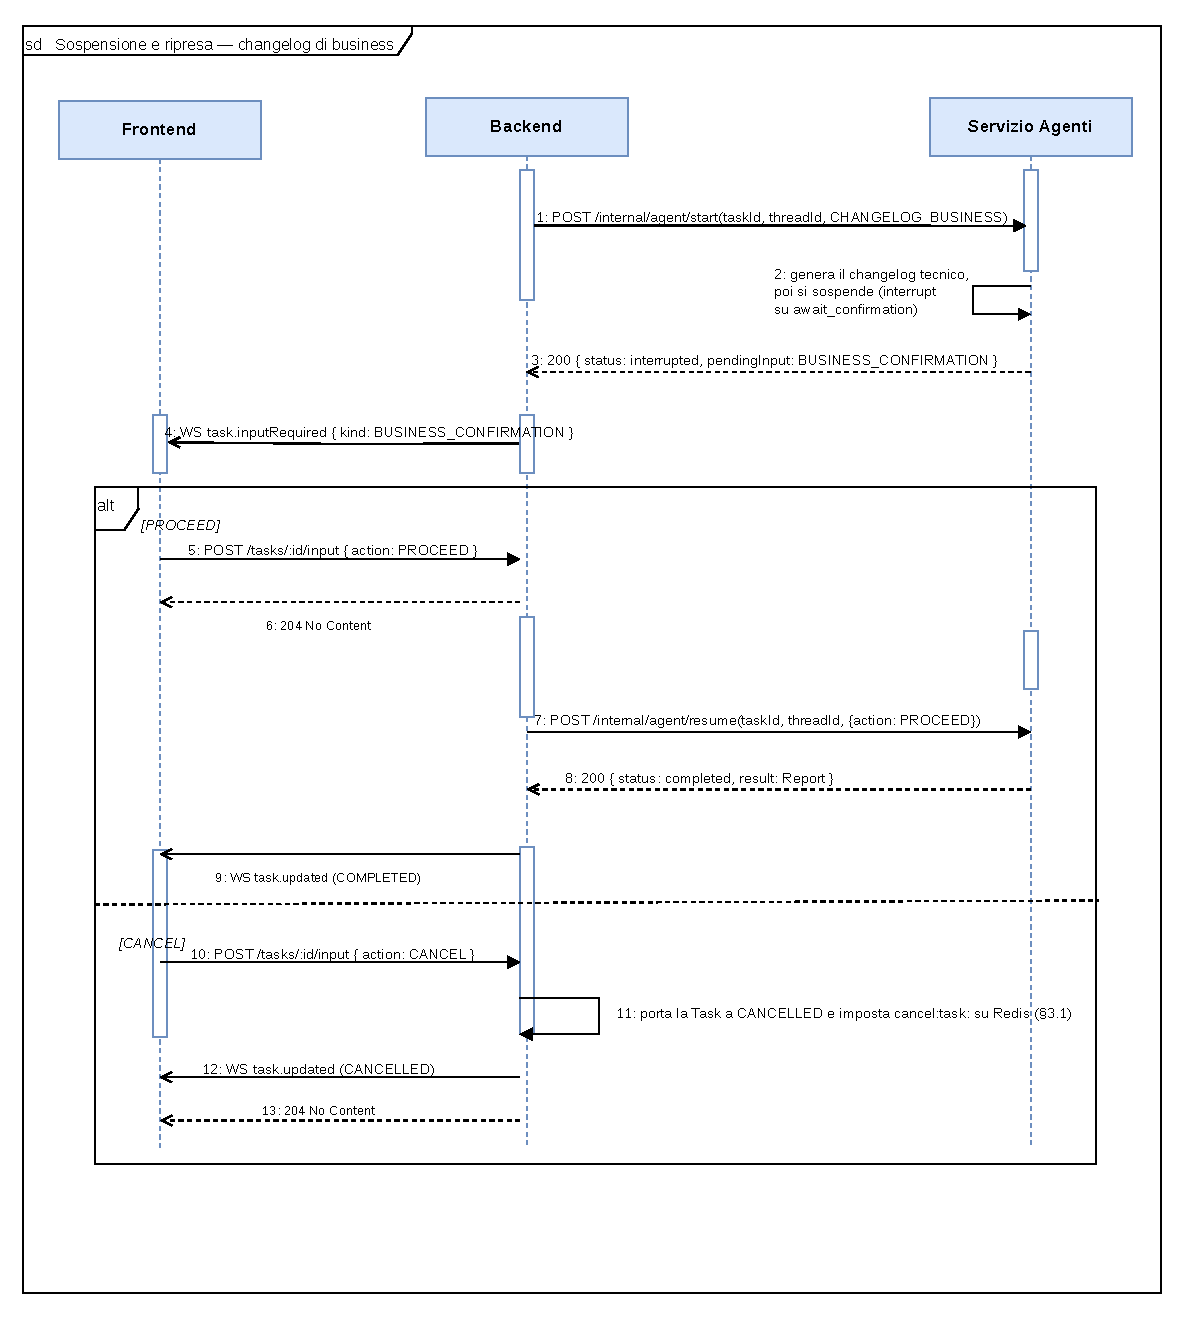
\includegraphics[width=1.0\textwidth]{changelog-sequenza-sospensione.pdf}
    \caption{Sospensione e ripresa dell'Agente Changelog.}
    \label{fig:flusso-sospensione}
\end{figure}

La chiamata che avvia l'esecuzione resta aperta per tutta la generazione del changelog tecnico, e si conclude solo quando il grafo si sospende: è per questo che il Backend riceve un esito di sospensione, e non una risposta separata, nel momento in cui la Task passa in attesa. La risposta dell'utente, in entrambi i rami, restituisce subito un \texttt{204} senza corpo; cosa succede dopo dipende dal ramo. Un rifiuto si esaurisce interamente e sincronamente dentro quella stessa richiesta: la Task passa a \texttt{CANCELLED}, viene impostato lo stesso flag Redis di cancellazione già descritto in \S~\ref{subsec:vista-insieme}, e l'evento \texttt{task.updated} parte prima ancora che il \texttt{204} torni al Frontend. Una conferma, invece, non richiama l'agente direttamente da quella richiesta: si limita ad accodare un nuovo job, con la stessa separazione tra richiesta ed esecuzione già vista nel primo scenario di questo capitolo. A invocare \texttt{/internal/agent/resume} è \texttt{TaskProcessor} quando preleva il job dalla coda, non il Backend che ha ricevuto la conferma.

\subsection{Esportazione di un Report in PDF}
\label{subsec:flusso-export}

L'ultimo scenario chiude il ciclo aperto dal primo: un Report completato può essere esportato in PDF.

\begin{figure}[H]
    \centering
    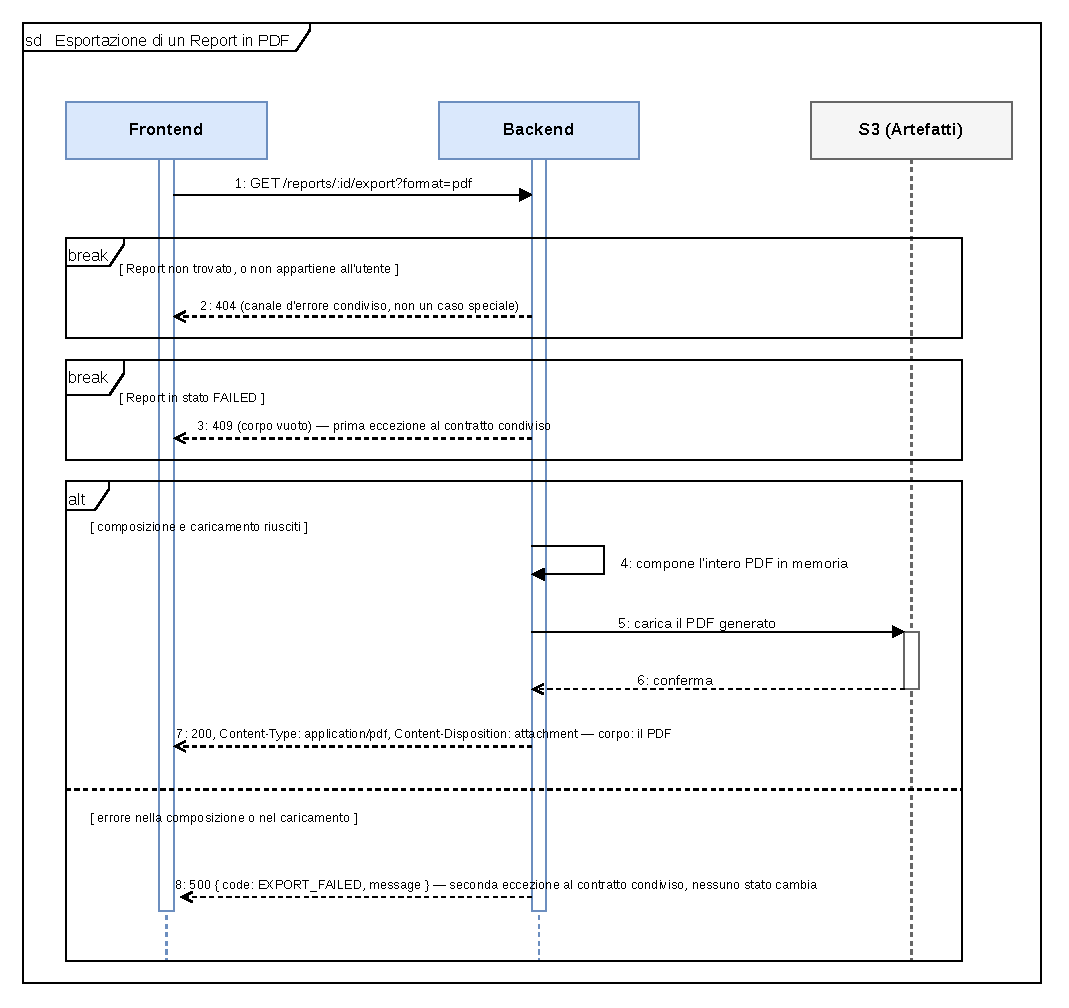
\includegraphics[width=1.0\textwidth]{flusso-esportazione-pdf.pdf}
    \caption{Esportazione di un Report in PDF.}
    \label{fig:flusso-export}
\end{figure}

Il PDF viene composto per intero in memoria prima che la risposta HTTP venga anche solo iniziata. Se la generazione fallisce a metà, nessun file parziale è già partito, perché nessuno stato \texttt{200} viene scritto finché non c'è un PDF completo da restituire. È anche l'unico scenario in cui il sistema tocca lo storage S3, dove l'artefatto generato viene caricato prima di essere restituito al Frontend. Un Report ancora in stato \texttt{FAILED} riceve invece un \texttt{409} a corpo vuoto, senza alcun tentativo di composizione: non esiste un PDF sensato da generare per un'analisi che non è mai arrivata a un risultato. Questo endpoint è poi l'unico a non seguire il contratto d'errore condiviso descritto altrove nel documento: un fallimento nella composizione o nel caricamento restituisce un corpo fisso \verb+{code: EXPORT\_FAILED, message}+. Abbiamo tenuto questo caso raro separato dal catalogo \texttt{error.code} che governa l'esecuzione delle Task.

\newpage
\section{Copertura dei requisiti}

I requisiti riportati in questa sezione sono quelli definiti nel documento \href{https://skynetunigroup.github.io/Code_Guardian/Documentazione/PB/analisi_dei_requisiti_v2.0.0.pdf}{Analisi dei Requisiti}, capitolo 7, e sono qui organizzati per sottosistema anziché nell'ordine in cui compaiono in quel documento. Per ciascun requisito le tabelle seguenti riportano il codice, la priorità e lo stato di soddisfacimento: \emph{Soddisfatto}, \emph{Parziale} se implementato solo in parte rispetto a quanto descritto, \emph{Non implementato} se non presente nell'MVP, oppure \emph{Fuori Perimetro} se abbiamo scelto di escluderlo dallo sviluppo, in accordo con il Proponente.

\subsection{Stato per requisito}

\medskip
\noindent\textbf{Identità, Autenticazione e Sicurezza Account}
\medskip

\begin{table}[H]
    \centering
    \renewcommand{\arraystretch}{1.3}
    \begin{tabular}{|c|c|c|}
        \hline
        \textbf{Codice} & \textbf{Priorità} & \textbf{Stato} \\ \hline
        RF.1--RF.9 & Obbligatorio & Soddisfatto \\ \hline
        RS.1 & Obbligatorio & Soddisfatto \\ \hline
    \end{tabular}
    \caption{Stato dei requisiti — Identità, Autenticazione e Sicurezza Account}
    \label{tab:req-identita}
\end{table}

\medskip
\noindent\textbf{Credenziali Esterne e Autorizzazione ai Servizi}
\medskip

\begin{table}[H]
    \centering
    \renewcommand{\arraystretch}{1.3}
    \begin{tabular}{|c|c|c|}
        \hline
        \textbf{Codice} & \textbf{Priorità} & \textbf{Stato} \\ \hline
        RF.10--RF.14 & Obbligatorio & Soddisfatto \\ \hline
        RS.2 & Obbligatorio & Soddisfatto \\ \hline
        RS.4 & Obbligatorio & Soddisfatto \\ \hline
    \end{tabular}
    \caption{Stato dei requisiti — Credenziali Esterne e Autorizzazione ai Servizi}
    \label{tab:req-credenziali}
\end{table}

\medskip
\noindent\textbf{Repository, Riferimento di Base e Ambito di Analisi}
\medskip

\begin{table}[H]
    \centering
    \renewcommand{\arraystretch}{1.3}
    \begin{tabular}{|c|c|c|}
        \hline
        \textbf{Codice} & \textbf{Priorità} & \textbf{Stato} \\ \hline
        RF.15--RF.17 & Obbligatorio & Soddisfatto \\ \hline
        RF.18 & Desiderabile & Fuori Perimetro \\ \hline
        RF.19--RF.22 & Obbligatorio & Soddisfatto \\ \hline
        RF.23 & Obbligatorio & Fuori Perimetro \\ \hline
        RF.24--RF.30 & Obbligatorio & Soddisfatto \\ \hline
        RF.31 & Desiderabile & Soddisfatto \\ \hline
        RQ.7 & Obbligatorio & Soddisfatto \\ \hline
        RQ.9--RQ.10 & Obbligatorio & Soddisfatto \\ \hline
    \end{tabular}
    \caption{Stato dei requisiti — Repository, Riferimento di Base e Ambito di Analisi}
    \label{tab:req-repository}
\end{table}

\medskip
\noindent\textbf{Selezione e Avvio delle Operazioni}
\medskip

\begin{table}[H]
    \centering
    \renewcommand{\arraystretch}{1.3}
    \begin{tabular}{|c|c|c|}
        \hline
        \textbf{Codice} & \textbf{Priorità} & \textbf{Stato} \\ \hline
        RF.32--RF.36 & Obbligatorio & Soddisfatto \\ \hline
        RF.37 & Desiderabile & Soddisfatto \\ \hline
        RF.38 & Opzionale & Fuori Perimetro \\ \hline
        RF.39 & Desiderabile & Soddisfatto \\ \hline
        RF.40--RF.42 & Obbligatorio & Soddisfatto \\ \hline
        RF.106 & Obbligatorio & Soddisfatto \\ \hline
    \end{tabular}
    \caption{Stato dei requisiti — Selezione e Avvio delle Operazioni}
    \label{tab:req-selezione}
\end{table}

\medskip
\noindent\textbf{Monitoraggio dell'Esecuzione}
\medskip

\begin{table}[H]
    \centering
    \renewcommand{\arraystretch}{1.3}
    \begin{tabular}{|c|c|c|}
        \hline
        \textbf{Codice} & \textbf{Priorità} & \textbf{Stato} \\ \hline
        RF.43--RF.48 & Obbligatorio & Soddisfatto \\ \hline
        RS.3 & Obbligatorio & Soddisfatto \\ \hline
    \end{tabular}
    \caption{Stato dei requisiti — Monitoraggio dell'Esecuzione}
    \label{tab:req-monitoraggio}
\end{table}

\medskip
\noindent\textbf{Storico e Archivio dei Report}
\medskip

\begin{table}[H]
    \centering
    \renewcommand{\arraystretch}{1.3}
    \begin{tabular}{|c|c|c|}
        \hline
        \textbf{Codice} & \textbf{Priorità} & \textbf{Stato} \\ \hline
        RF.49--RF.52 & Opzionale & Soddisfatto \\ \hline
    \end{tabular}
    \caption{Stato dei requisiti — Storico e Archivio dei Report}
    \label{tab:req-storico}
\end{table}

\medskip
\noindent\textbf{Visualizzazione e Struttura del Report}
\medskip

\begin{table}[H]
    \centering
    \renewcommand{\arraystretch}{1.3}
    \begin{tabular}{|c|c|c|}
        \hline
        \textbf{Codice} & \textbf{Priorità} & \textbf{Stato} \\ \hline
        RF.53--RF.56 & Obbligatorio & Soddisfatto \\ \hline
        RF.57--RF.61 & Obbligatorio & Soddisfatto \\ \hline
        RF.62--RF.63 & Obbligatorio & Soddisfatto \\ \hline
        RF.64 & Obbligatorio & Parziale \\ \hline
        
        %%%% 62 implementato, 64 non imp, 63 imp.
    \end{tabular}
    \caption{Stato dei requisiti — Visualizzazione e Struttura del Report}
    \label{tab:req-visualizzazione}
\end{table}

\medskip
\noindent\textbf{Gestione degli Errori di Esecuzione}
\medskip

\begin{table}[H]
    \centering
    \renewcommand{\arraystretch}{1.3}
    \begin{tabular}{|c|c|c|}
        \hline
        \textbf{Codice} & \textbf{Priorità} & \textbf{Stato} \\ \hline
        RF.65 & Obbligatorio & Soddisfatto \\ \hline
        RF.66--RF.67 & Desiderabile & Soddisfatto \\ \hline
        RF.68--RF.72 & Obbligatorio & Soddisfatto \\ \hline
    \end{tabular}
    \caption{Stato dei requisiti — Gestione degli Errori di Esecuzione}
    \label{tab:req-errori}
\end{table}

\medskip
\noindent\textbf{Esportazione e Notifiche}
\medskip

\begin{table}[H]
    \centering
    \renewcommand{\arraystretch}{1.3}
    \begin{tabular}{|c|c|c|}
        \hline
        \textbf{Codice} & \textbf{Priorità} & \textbf{Stato} \\ \hline
        RF.73--RF.74 & Obbligatorio & Soddisfatto \\ \hline
        RF.75--RF.78 & Opzionale & Fuori Perimetro \\ \hline
    \end{tabular}
    \caption{Stato dei requisiti — Esportazione e Notifiche}
    \label{tab:req-esportazione}
\end{table}

\medskip
\noindent\textbf{Agente Docs}
\medskip

\begin{table}[H]
    \centering
    \renewcommand{\arraystretch}{1.3}
    \begin{tabular}{|c|c|c|}
        \hline
        \textbf{Codice} & \textbf{Priorità} & \textbf{Stato} \\ \hline
        RF.79--RF.81 & Opzionale & Soddisfatto \\ \hline
        RF.82--RF.84 & Obbligatorio & Soddisfatto \\ \hline
        RF.85 & Desiderabile & Non implementato \\ \hline
        RF.86 & Obbligatorio & Soddisfatto \\ \hline
    \end{tabular}
    \caption{Stato dei requisiti — Agente Docs}
    \label{tab:req-docs}
\end{table}

\medskip
\noindent\textbf{Agente Security}
\medskip

\begin{table}[H]
    \centering
    \renewcommand{\arraystretch}{1.3}
    \begin{tabular}{|c|c|c|}
        \hline
        \textbf{Codice} & \textbf{Priorità} & \textbf{Stato} \\ \hline
        RF.87--RF.91 & Obbligatorio & Soddisfatto \\ \hline
        RF.92 & Obbligatorio & Soddisfatto \\ \hline
        RF.93 & Obbligatorio & Non implementato \\ \hline
    \end{tabular}
    \caption{Stato dei requisiti — Agente Security}
    \label{tab:req-security}
\end{table}

\medskip
\noindent\textbf{Agente Changelog e Task Management}
\medskip

\begin{table}[H]
    \centering
    \renewcommand{\arraystretch}{1.3}
    \begin{tabular}{|c|c|c|}
        \hline
        \textbf{Codice} & \textbf{Priorità} & \textbf{Stato} \\ \hline
        RF.94 & Obbligatorio & Soddisfatto \\ \hline
        RF.95 & Obbligatorio & Parziale \\ \hline
        RF.96 & Obbligatorio & Soddisfatto \\ \hline
        RF.97 & Opzionale & Soddisfatto \\ \hline
        RF.98--RF.99 & Obbligatorio & Soddisfatto \\ \hline
        RF.100 & Obbligatorio & Parziale \\ \hline
        RF.101--RF.105 & Obbligatorio & Soddisfatto \\ \hline
        RF.108 & Obbligatorio & Soddisfatto \\ \hline
        RQ.11 & Obbligatorio & Soddisfatto \\ \hline
    \end{tabular}
    \caption{Stato dei requisiti — Agente Changelog e Task Management}
    \label{tab:req-changelog}
\end{table}

\medskip
\noindent\textbf{Prestazioni e Limiti Operativi}
\medskip

\begin{table}[H]
    \centering
    \renewcommand{\arraystretch}{1.3}
    \begin{tabular}{|c|c|c|}
        \hline
        \textbf{Codice} & \textbf{Priorità} & \textbf{Stato} \\ \hline
        RF.107 & Obbligatorio & Soddisfatto \\ \hline
        RF.109--RF.110 & Desiderabile & Soddisfatto \\ \hline
        RF.111 & Obbligatorio & Soddisfatto \\ \hline
        RQ.8 & Desiderabile & Soddisfatto \\ \hline
    \end{tabular}
    \caption{Stato dei requisiti — Prestazioni e Limiti Operativi}
    \label{tab:req-prestazioni}
\end{table}

\medskip
\noindent\textbf{Vincoli Tecnologici e Infrastrutturali}
\medskip

\begin{table}[H]
    \centering
    \renewcommand{\arraystretch}{1.3}
    \begin{tabular}{|c|c|c|}
        \hline
        \textbf{Codice} & \textbf{Priorità} & \textbf{Stato} \\ \hline
        RV.1--RV.8 & Obbligatorio & Soddisfatto \\ \hline
        RS.5 & Desiderabile & Parziale \\ \hline
    \end{tabular}
    \caption{Stato dei requisiti — Vincoli Tecnologici e Infrastrutturali}
    \label{tab:req-vincoli}
\end{table}

\medskip
\noindent\textbf{Qualità del Codice, Test e Affidabilità AI}
\medskip

\begin{table}[H]
    \centering
    \renewcommand{\arraystretch}{1.3}
    \begin{tabular}{|c|c|c|}
        \hline
        \textbf{Codice} & \textbf{Priorità} & \textbf{Stato} \\ \hline
        RQ.1--RQ.2 & Obbligatorio & Soddisfatto \\ \hline
        RQ.3 & Obbligatorio & Non implementato \\ \hline
        RQ.4 & Obbligatorio & Soddisfatto \\ \hline
        RQ.5 & Obbligatorio & Non implementato \\ \hline
        RQ.6 & Obbligatorio & Fuori perimetro \\ \hline
    \end{tabular}
    \caption{Stato dei requisiti — Qualità del Codice, Test e Affidabilità AI}
    \label{tab:req-qualita-codice}
\end{table}

\medskip
\noindent\textbf{Qualità di Processo e Documentazione di Progetto}
\medskip

\begin{table}[H]
    \centering
    \renewcommand{\arraystretch}{1.3}
    \begin{tabular}{|c|c|c|}
        \hline
        \textbf{Codice} & \textbf{Priorità} & \textbf{Stato} \\ \hline
        RQ.12--RQ.16 & Obbligatorio & Soddisfatto \\ \hline
        RQ.17 & Obbligatorio & Parziale \\ \hline
    \end{tabular}
    \caption{Stato dei requisiti — Qualità di Processo e Documentazione di Progetto}
    \label{tab:req-qualita-processo}
\end{table}

\subsection{Percentuali di riepilogo}


\begin{table}[H]
    \centering
    \renewcommand{\arraystretch}{1.3}
    \begin{tabular}{|l|*{4}{>{\centering\arraybackslash}p{2.7cm}|}}
        \hline
        \textbf{Categoria} & \textbf{\% soddisfatta} & \textbf{\% parziale} & \textbf{\% non implementata} & \textbf{\% fuori perimetro} \\ \hline
        Requisiti Funzionali & 89,2 & 2,7 & 1,8 & 6,3 \\ \hline
        Requisiti Qualitativi & 76,4 & 5,9 & 11,8 & 5,9 \\ \hline
        Requisiti di Vincolo & 100 & 0 & 0 & 0 \\ \hline
        Requisiti di Sicurezza & 80 & 20 & 0 & 0 \\ \hline
        Requisiti Desiderabili & 72,3 & 9,1 & 9,1 & 9,1 \\ \hline
        Requisiti Opzionali & 100 & 0 & 0 & 0 \\ \hline
        Requisiti Obbligatori & 92,3 & 3,4 & 2,6 & 1,7 \\ \hline
    \end{tabular}
    \caption{Percentuali di riepilogo dello stato dei requisiti}
    \label{tab:req-percentuali}
\end{table}

\end{document}
